% !TEX root = ../main.tex
\documentclass[../main.tex]{subfiles}
\begin{document}

\appendix

% Appendices of every chapter, gathered here in chapter order. Labels keep their
% original per-chapter prefix, so cross references from the chapters still resolve.

\chapter{Internal Tide-Eddy Interactions and the Formation of Internal Wave Continuum}
\begingroup
% Paper-specific macros for the Internal Tide-Eddy chapter and its appendix.
% Always \input inside a \begingroup..\endgroup so they cannot leak into other
% chapters' math, since several of these names are also used with different
% meanings elsewhere, e.g. \grad, \div, \hat, \bar.
% Macros the chapter never called were removed; the original paper keeps them.
\renewcommand{\hat}{\widehat}
\newcommand{\p}{\partial}
\newcommand{\bs}[1]{\boldsymbol{#1}}
\renewcommand{\del}{\nabla}
\newcommand{\bsh}[1]{\boldsymbol{\hat{#1}}}
\newcommand{\dd}[2]{\frac{d{#1}}{d{#2}}}
\renewcommand{\bar}[1]{\overline{#1}}
\renewcommand{\t}[1]{\widetilde{#1}}
\renewcommand{\grad}[1]{\del#1}
\renewcommand{\div}[1]{\del . {#1}}


\section{Orthogonality of linear geostrophic-ageostrophic decomposition}\label{edwv-budet}

%Equations \eqref{edwv-pv},\eqref{edwv-ug} can be summarized by expressing the geostrophic flow as a projection on the net flow by a projection operator $\mb{P}$, i.e.

The linear geostrophic-ageostrophic decomposition we employed is similar to that used in several past studies in different configurations \citep{Bartello95, Embid_Majda_1998, Hernandez_Smith_Stechmann_2014, TD20, RT26}. This decomposition can be written as the projection of the full fields on to the geostrophic and the ageostrophic flow with a projection operator $\mb{P}$ as, 
\begin{align}
\label{edwv-buprj}
\begin{split}
 \begin{bmatrix}
 u_g \\
 v_g \\
 w_g \\
 b_g \\
 \end{bmatrix}= \mb{P}
 \begin{bmatrix}
 u \\
 v \\
 w \\
 b \\
 \end{bmatrix}, \quad\mbox{ where} \quad 
 \mb{P} = \begin{bmatrix}
 -\frac{\partial}{\partial y} \\
 \frac{\partial}{\partial x} \\
 0\\
 \frac{\partial}{\partial z}
 \end{bmatrix}\Delta^{-1}
 \begin{bmatrix}
 -\frac{\partial}{\partial y},\frac{\partial}{\partial x},0,\frac{\partial}{\partial z} 
 \end{bmatrix}, \quad \mbox{ and} \quad 
	\begin{bmatrix}
		u_a \\
		v_a \\
		w_a \\
		b_a \\
	\end{bmatrix}= \left( \mb{I}_{4} - \mb{P} \right)
	\begin{bmatrix}
		u \\
		v \\
		w \\
		b \\
	\end{bmatrix} \ ,
\end{split}
\end{align}
where $\mb{I}_4$ is the $4$ dimensional identity matrix. The equivalent relations in the spectral space for \eqref{edwv-buprj} is 
\begin{align}
\label{edwv-sbuprj}
\begin{split}
 \begin{bmatrix}
 \hat{u}_g \\
 \hat{v}_g \\
 \hat{w}_g \\
 \hat{b}_g \\
 \end{bmatrix}= \hat{\mb{P}}
 \begin{bmatrix}
 \hat{u} \\
 \hat{v} \\
 \hat{w} \\
 \hat{b} \\
 \end{bmatrix} \quad , \quad
		\hat{\mb{P}} = -\frac{1}{k_h^2 + k_z^2}\begin{bmatrix}
 -ik_y \\
 ik_x \\
 0\\
 -k_z
 \end{bmatrix}
 \begin{bmatrix}
 -ik_y,ik_x,0,k_z
 \end{bmatrix},\quad \mbox{ and} \quad
	\begin{bmatrix}
 \hat{u}_a \\
 \hat{v}_a \\
 \hat{w}_a \\
 \hat{b}_a \\
 \end{bmatrix}= \left( \mb{I}_{4} - \hat{\mb{P}} \right)
 \begin{bmatrix}
 \hat{u} \\
 \hat{v} \\
 \hat{w} \\
 \hat{b} \\
 \end{bmatrix} , 
\end{split}
\end{align}
where $\hat{.}$ denotes quantities in spectral space. From the definition in \eqref{edwv-sbuprj}, $\hat{\mb{P}}^{\dagger} = \hat{\mb{P}}^2 = \hat{\mb{P}}$. The net energy at each wavevector $(\vec{k}_h , k_z)$ is given by 
\begin{align}
 \label{edwv-e3d}
 \begin{split}
 \hat{e}\left( \vec{k}_h, k_z,t \right) = \frac{1}{2}\left( |\hat{u}|^2 + |\hat{v}|^2 + \frac{|\hat{w}|^2}{\AR^2} + |\hat{b}|^2\right) \ ,
 \end{split}
\end{align}
And upon splitting the net flow into geostrophic and ageostrophic components, we get 
\begin{align}
 % \label}
 \begin{split}
 \hat{e}\left( \vec{k}_h, k_z,t \right) =& \hat{e}_g\left( \vec{k}_h, k_z,t \right) + \hat{e}_a\left( \vec{k}_h, k_z,t \right)+ \op{Re}\left( \hat{u}_g^* \hat u_a + \hat{v}_g^* \hat v_a + \frac{\hat{w}_g^* \hat w_a}{\AR^2} + \hat{b}_g^* \hat b_a\right) \ , 
 \end{split}
\end{align}
where $\hat{e}_g$ and $\hat{e}_a$ are the geostrophic and ageostrophic energy at wavenumber $(\vec{k}_h, k_z)$ with the definition given in \eqref{edwv-e3d}. Noting $\hat{w}_g = 0$, the cross terms in the energy vanish using \eqref{edwv-sbuprj}, 
\begin{align}
 % \label{}
 \begin{split}
 \hat{u}_g^* \hat u_a + \hat{v}_g^* \hat v_a + \frac{\hat{w}_g^* \hat w_a}{\AR^2} + \hat{b}_g^* \hat b_a = \begin{bmatrix}
 \hat{u}_g^*,\hat{v}_g^*,\hat{w}_g^*, \hat{b}_g^*
 \end{bmatrix} \begin{bmatrix}
 \hat{u}_a \\
 \hat{v}_a \\
 \hat{w}_a \\
 \hat{b}_a \\
 \end{bmatrix} = \begin{bmatrix}
 \hat{u}^*,\hat{v}^*,\hat{w}^*, \hat{b}^*
 \end{bmatrix}\hat{\mb{P}} \left(\mb{I}_4 - \hat{\mb{P}}^\dagger\right) \begin{bmatrix}
 \hat{u} \\
 \hat{v} \\
 \hat{w} \\
 \hat{b} \\
 \end{bmatrix} = 0 \ .
 \end{split}
\end{align}

Above result implies that the net energy of the flow  splits exactly into contributions  from the geostrophic and the ageostrophic components at each wavenumber, without any cross terms. In other words, the linear decomposition above is an orthogonal one. We used this property to split the energy and the spectral flux of the net flow into geostrophic and ageostrophic components.

\section{Orthogonality of the slow-fast decomposition}\label{edwv-sfdet}

The orthogonality of geostrophic-ageostrophic components shown in appendix \ref{edwv-budet} does not hold for the slow-fast decomposition. Specifically, the slow and fast components are only orthogonal in the frequency domain. Thus, for any two real functions $\psi(t)$ and $\phi(t)$, we have
\begin{equation}
    \label{edwv-sff}
    \hat{\psi}_f(\omega) \hat{\phi}_s(\omega) = \hat{\psi}_s(\omega) \hat{\phi}_f(\omega) = 0
\end{equation} 
Since we use  a sharp frequency filter, the fast field has no slow frequency components while the slow field has no high frequency components. This lack of overlap leads to perfect orthogonality in the frequency domain, although it does not translate to the time domain, i.e. $\psi_s(t)\phi_f(t)\neq 0 \neq \psi_f(t)\phi_s(t)$. Nevertheless, from Parseval's theorem, we have 
\begin{align}
 % \label{}
 \begin{split}
 \int \frac{1}{2\pi} \op{Re}\left[\hat{\psi}^*(\omega) \hat{\phi}(\omega) \right] d\omega = \int \psi(t)\phi(t) dt \ .
 \end{split}
\end{align}
Therefore, we have 
\begin{align}
 \label{edwv-sforth}
 \begin{split}
 \int \phi_s(t)\psi_f(t) dt= \int\frac{1}{2\pi} \op{Re}\left[\hat{\psi}_f^*(\omega) \hat{\phi}_s(\omega) \right] d\omega &= 0 \\ 
 \int \phi_f(t)\psi_s(t) dt= \int\frac{1}{2\pi} \op{Re}\left[\hat{\psi}_s^*(\omega) \hat{\phi}_f(\omega) \right] d\omega &= 0 \ .
 \end{split}
\end{align}

The above expressions apply to functions in the frequency domain. When functions are sampled over $N_t$ points between time instances $t_i$ and $t_f$, we are forced to use a discrete Fourier transform. In that case, the analogous equations to \eqref{edwv-sforth} will be
\begin{align}
 \label{edwv-sfft}
 \begin{split}
 \delta t\sum\limits_{t_i}^{t_f} \phi_s(t_s)\psi_f(t_s) = \frac{\delta \omega}{2\pi}\sum\limits_{-\omega_{\op{max}}}^{\omega_{\op{max}}} \op{Re}\left[\hat{\psi}_f^*(\omega) \hat{\phi}_s(\omega) \right] &= 0 \\
 \delta t\sum\limits_{t_i}^{t_f} \phi_f(t_s)\psi_s(t_s) = \frac{\delta \omega}{2\pi}\sum\limits_{-\omega_{\op{max}}}^{\omega_{\op{max}}} \op{Re}\left[\hat{\psi}_s^*(\omega) \hat{\phi}_f(\omega) \right] &= 0 \ ,
\end{split}
\end{align}
where $\omega_{\op{max}} = \pi N_t/(t_f - t_i)$ is the maximum frequency resolved by a discrete Fourier transform, and $\delta t = (t_f - t_i)/N_t$ and $\delta \omega = 2\pi/(t_f - t_i)$ are the sampling intervals of time and frequency respectively. This tells us that the fast and the slow components of the flow can be orthogonal, but only in a time-integrated or time-averaged sense. We used the above features to get the spectral energy distribution and spectral flux for slow and fast components. 

 
\section{Forcing of the geostrophic and the tidal flow}\label{edwv-fdets}
This section details the method of forcing implemented in the numerical simulation to obtain energy ratios $E_g/E_a= 8,1$. We force the geostrophic and the ageostrophic flow separately. For both the geostrophic and the ageostrophic flow, the pressure field specifies the entire flow.
\subsection{Geostrophic forcing}
Specifying a geostrophic pressure $f_{p_g}$, the geostrophic velocity field is given by 
\begin{align}
% \label{}
\begin{split}
	\vec{f}_{v_g} = \bsh z \times \grad{f_{p_g}}\qquad; \qquad f_{w_g} = 0 \qquad,\mbox{ and}\qquad f_{b_g} = \frac{\partial f_{p_g}}{\partial z} \ .
\end{split}
\end{align}
Thus, to force the geostrophic flow, we initialize a pressure field $f_{p_g}$ in the spectral space with $k = \sqrt{k_h^2 + k_z^2}< 6$, and define the geostrophic forcing $\vec{f}_{v_g}, \ f_{w_g}, \  f_{b_g}$ as 
\begin{align}
% \label{}
\begin{split}
	\Big(\vec{F}_{v_g},F_{w_g}, F_{b_g}\Big)(x,y,z,t) = A_g\Big(\vec{f}_{v_g},0,f_{b_g}\Big)(x,y,z)\Theta\left(E_c^g - E_g(t)\right) \ ,
\end{split}
\end{align}
where $E_g(t)$ is the instantaneous geostrophic energy of the flow field and $A_g$is the amplitude of the forcing. $E_c^g =4$ is the critical energy above which the geostrophic forcing vanishes. 


\subsection{Ageostrophic forcing}
We followed a similar prescription for the tidal forcing. Given, an ageostrophic pressure field $\hat{f}_{p_a}$ in the spectral space, a plane wave solution of the linear inviscid part  of \eqref{edwv-bsnq} satisfies
\begin{align}
\label{edwv-linwv}
\begin{split}
	\hat{f}_{u_a} = \hat{f}_{p_a}\ \frac{ ik_y + k_x\,\omega}{\omega^2 -1}\quad &; \quad \hat{f}_{v_a}= \hat{f}_{p_a}\ \frac{-i k_x + k_y\,\omega}{\omega^2 -1} \\
	\hat{f}_{w_a} =-i \hat{f}_{p_a}\ \frac{ \omega k_h^2}{k_z \left( \omega^2 -1 \right)} \quad &; \quad \hat{f}_{b_a} = - \hat{f}_{p_a} \ \frac{ k_h^2}{k_z \left( \omega^2 -1 \right)} \ , 
\end{split}
\end{align}
with $k_h = \sqrt{k_x^2 + k_y^2} = \sqrt{2}$, $k_z = 1$, and $\omega=\omega_0 = 1.73$, the forcing frequency,  from the linear wave dispersion relation. Using this, the ageostrophic forcing in spectral space becomes 
\begin{align}
% \label{}
\begin{split}
	\begin{bmatrix}
		\hat{F}_{u_a}\\
		\hat{F}_{v_a}\\
		\hat{F}_{w_a}\\
		\hat{F}_{b_a}\\
	\end{bmatrix}(\vec{k}_h,k_z,t) = A_a \begin{bmatrix}
		\hat{f}_{u_a}(\vec{k}_h, k_z,t) + \left(\hat{f}_{u_a}(-\vec{k}_h, k_z,t)\right)^*\\
		\hat{f}_{v_a}(\vec{k}_h, k_z,t) + \left(\hat{f}_{v_a}(-\vec{k}_h, k_z,t)\right)^*\\
		\hat{f}_{w_a}(\vec{k}_h, k_z,t) + \left(\hat{f}_{w_a}(-\vec{k}_h, k_z,t)\right)^*\\
		\hat{f}_{b_a}(\vec{k}_h, k_z,t) + \left(\hat{f}_{b_a}(-\vec{k}_h, k_z,t)\right)^*\\
	\end{bmatrix} \cos(\omega t)\mathcal H \left(E_c^a - E_a(t)\right) \ ,
\end{split}
\end{align}
where we use the complex conjugate part of each field to ensure that the forcing is real in physical space.    $A_a$ is the wave forcing amplitude and  the threshold energy $E_c^a$ was set to $0.5$ and $4$ for $E_g/E_a = 8$ and 1 cases, respectively.



\section{Filtered energy budget equation}\label{edwv-fluxeqn}

Here, we will derive the spatially filtered energy evolution equation. For convenience, we scale our vertical coordinate $z$ as
\begin{align}
 % \label{}
 \begin{split}
 z \to \frac{z}{\AR} \ .
 \end{split}
\end{align}
This changes the vertical velocity and the vertical derivative to
\begin{align}
 % \label{}
 \begin{split}
 w \to \frac{w}{\AR} \qquad ; \qquad \Dp{}{z}{}\to \AR \Dp{}{z}{} .
 \end{split}
\end{align}

With the above scalings, the Boussinesq equations in \eqref{edwv-bsnq}, in the absence of forcing and dissipation, become
\begin{align}
 \label{edwv-bsnqsc}
 \begin{split}
 \Dp{u_i}{t}{}+ Ro~ u_k\Dp{ u_i}{x_k}{}+ \epsilon_{i3k} u_k &= - \Dp{\mathcal{P}}{x_i}{} + \AR b \delta_{3i} \\
 \Dp{b}{t}{} + Ro~ u_k\Dp{b}{x_k}{} &= - \AR w \\
 \Dp{u_i}{x_i}{} &= 0 \ ,
 \end{split}
\end{align}
where $\vec{u} = (u,v,w)$ is the full three dimensional velocity. Above, we used Einstein's summation convention where quantities with repeated indices are summed over their components, $x,y$, and $z$, and $\delta_{ij}$ is the Kronecker delta function. Next, we define the large-scale component of the flow using a filter on an arbitrary flow variable $\phi$ as $\t{\phi} = \phi - \phi'$, where $\phi'$ is the remaining small-scale flow variable. The filters are defined such that they commute with spatial and time derivatives
\begin{align}
 % \label{}
 \begin{split}
 \t{\Dp{\phi}{t}{}} = \Dp{\t{\phi}}{t}{} \ ; \ \t{\Dp{\phi}{x_i}{}} = \Dp{\t{\phi}}{x_i}{} \ . 
 \end{split}
\end{align}
Applying the filter on \eqref{edwv-bsnqsc} gives us large-scale flow evolution equations as 
\begin{align}
\label{edwv-feq}
 \begin{split}
 \Dp{\t{u_i}}{t}{}+ Ro~ \t{u_k\Dp{ u_i}{x_k}{}}+ \epsilon_{i3k} \t{u}_k &= - \Dp{\t{\mathcal{P}}}{x_i}{} + \AR \t{b} \delta_{3i} \\
 \Dp{\t{b}}{t}{} + Ro~ \t{u_k\Dp{b}{x_k}{}} &= - \AR \t{w} \\
 \Dp{\t{u}_i}{x_i}{} &= 0 \ ,
 \end{split}
\end{align}
where $u_i$ forms a component of the three-dimensional velocity in the scaled coordinate system, and $\epsilon_{ijk}$ is the  Levi-Civita tensor. The large-scale energy of the flow is given by
\begin{align}
 % \label{}
 \begin{split}
 \t{e} = \frac{1}{2}\left(\t{u}_i \t{u}_i + \t{b}~\t{b} \right) \ , 
 \end{split}
\end{align}
and we can get an evolution equation of $\t{e}$ by summing the dot product of the velocity equation in \eqref{edwv-feq} with $\tilde u_i$ and buoyancy equation in \eqref{edwv-feq} with $\tilde b_i$. The energy equation so obtained is 
\begin{align}
 % \label{}
 \begin{split}
 \Dp{ \t{e}}{t}{} + Ro\,\Dp{}{x_k}{} \left(\t{u}_k \t{e}\right) = &Ro\, \left[\t{u}_k \Dp{}{x_j}{} \left(\t{u}_j\t{u}_k - \t{u_j u_k}\right)\right]+ Ro\left[\t{b} \Dp{}{x_k}{} (\t{u}_k\t{b} - \t{b u_k})\right] - \Dp{}{x_k}{}(\t{u}_k\t{\mathcal{P}}) \ .
 \end{split}
\end{align}
Rearranging the above terms using 
\begin{align}
 \label{edwv-lstrs}
 \begin{split}
 \tau_{ij} = \t{u}_i \t{u}_j - \t{u_i u_j} \quad ;\quad B_k = \t{u}_k\t{b} - \t{b u_k} \ ,
 \end{split}
\end{align}
gives us 
\begin{align}
 % \label{}
 \begin{split}
 \Dp{\t{e}}{t}{} + Ro\,\Dp{}{x_k}{}\left(\t{u}_k \t{e}\right) = &-Ro\left[- \tau_{jk}\Dp{\t{u}_j }{x_k}{}- B_k\Dp{\t{b}}{x_k}{} + \Dp{}{x_k}{}\left(\tau_{jk} \t{u}_j + B_k \t{b}\right) \right]  - \Dp{}{x_k}{}(\t{u}_k\t{\mathcal{P}}) \ .
 \end{split}
\end{align}
Further rearranging gives us 
\begin{align}
 \label{edwv-sclflux}
 \begin{split}
 \Dp{\t{e}}{t}{} + Ro\,\Dp{}{x_k}{} \left[\t{u}_j \left(\left(\t{e}+\frac{\t{\mathcal{P}}}{Ro}\right)\delta_{jk} - \tau_{jk}\right) - B_k \t{b}\right] = &-Ro ~\tau_{jk}\Dp{\t{u}_j}{x_k}{} - Ro~B_k\Dp{\t{b}}{x_k}{} \ .
 \end{split}
\end{align}
The right-hand side of the above equation does not vanish when integrated over the spatial domain and is responsible for the cross-scale energy transfer. Rescaling back to the original variables leads to the filtered energy equation given in \eqref{edwv-ebdg}.
\endgroup

\chapter{Caustics of finitely dense inertial particles}

\section{Derivation of caustics condition for frozen caustics} \label{int-caus-reg-drv}
To obtain \eref{int-caus_cond}, we extend the procedure outlined by \cite{meibohm2023} to the case of $\alpha \ne 1$. Defining the independent invariants of $\mb{A}$ and $\mb{Z}$ as
\begin{align}
\begin{split}
  a = \Tr{\mb{A}} = 0; \quad Q = -\frac{1}{2}\Tr{\mb{A}^2}; \quad R = - \det{\mb{A}} = -\frac{1}{3}\Tr{\mb{A}^3};
\quad z_2 = \Tr{\mb{Z}^2}; \quad \mathfrak{d} =  \det{\mb{Z}},
\end{split}
\end{align}
we can write coupled algebraic equations for $\delta,z_2,\text{ and }\mathfrak{d}$ in terms of $Q$ and $R$ by taking different powers of \eref{int-root-eq}, taking their trace, and using Cayley-Hamilton theorem. Further, eliminating $z_2$ and $\mathfrak{d}$, and defining  $\delta \equiv \pm \sqrt{\chi} - 3\alpha/2$, we get, after some algebra
\begin{align}
\begin{split}
   & \left(\chi^2 + \frac{a_2 }{2}\chi + a_0\right)^2 +  \chi\left(a_1 - a_2a_0\right) = 0, \quad {\rm where} \label{int-pol4}\\
    a_0 &=  -\frac{3 \alpha ^4}{16}-(3 \alpha +1) \alpha ^2 Q+36 (\alpha -1) \alpha  R, \\
    a_1 &=-\frac{7 \alpha ^6}{16}-24 (7-3 \alpha ) (1-\alpha ) \alpha ^2 Q^2-\frac{1}{2} (21 \alpha -13) \alpha ^4 Q-288 (1-\alpha )^2 \alpha  Q R\\&\mathrel{\phantom{ =} }-1728 (1-\alpha )^3 R^2+4 (9 \alpha +7) \alpha ^3 R, \quad
    {\rm } \ a_2 = 3 \left[8 (1-\alpha ) Q-\alpha ^2\right]\ .
\end{split}
\end{align}
The condition for caustics reduces to not having any positive root of $\chi$ in \eref{int-pol4}. This happens when $a_1 - a_2a_0 > 0$, which yields \eref{int-caus_cond}.

\chapter{Active Caustics}

\section{Supplementary Videos}
\label{act-videos}
\textbf{\href{https://office365stanford-my.sharepoint.com/:v:/g/personal/rchajwa_stanford_edu/EU2dPLsDJGVOjePmOh_22aEBiQbmSoQjO7OQmnt6cHVS6g?nav=eyJyZWZlcnJhbEluZm8iOnsicmVmZXJyYWxBcHAiOiJPbmVEcml2ZUZvckJ1c2luZXNzIiwicmVmZXJyYWxBcHBQbGF0Zm9ybSI6IldlYiIsInJlZmVycmFsTW9kZSI6InZpZXciLCJyZWZlcnJhbFZpZXciOiJNeUZpbGVzTGlua0NvcHkifX0&e=M0zgMJ}{Video 1}:} Active Hookean dimers with $\alpha_{\rm act} =1$, $l = 0$ in a point vortex flow. It is compared with the dynamics of inertial particles.

\textbf{\href{https://office365stanford-my.sharepoint.com/:v:/g/personal/rchajwa_stanford_edu/EXS4TQknhbJIkFp9oUu78FUBwCOYzjiOakzS09ai0bqH8Q?nav=eyJyZWZlcnJhbEluZm8iOnsicmVmZXJyYWxBcHAiOiJPbmVEcml2ZUZvckJ1c2luZXNzIiwicmVmZXJyYWxBcHBQbGF0Zm9ybSI6IldlYiIsInJlZmVycmFsTW9kZSI6InZpZXciLCJyZWZlcnJhbFZpZXciOiJNeUZpbGVzTGlua0NvcHkifX0&e=VLAmFk}{Video 2}:} Active Preferred-length dimers with $\alpha_{\rm act} =1$, $l = 0$, $\beta \sqrt{\tau_{\rm act}/\Gamma} = 0.5$ in a point vortex flow.

\textbf{\href{https://office365stanford-my.sharepoint.com/:v:/g/personal/rchajwa_stanford_edu/EVu_8SMbr4xCo9drLsQOrsABtEuOLzmdwRygR-g2_Q2tXw?nav=eyJyZWZlcnJhbEluZm8iOnsicmVmZXJyYWxBcHAiOiJPbmVEcml2ZUZvckJ1c2luZXNzIiwicmVmZXJyYWxBcHBQbGF0Zm9ybSI6IldlYiIsInJlZmVycmFsTW9kZSI6InZpZXciLCJyZWZlcnJhbFZpZXciOiJNeUZpbGVzTGlua0NvcHkifX0&e=baRa3i}{Video 3}:} Preferred-length dimers in turbulence with flow parameters given by Table I of methods section, and with $\alpha_{\rm act} = 1$, $\tau_{\rm act} = 1$,  $l^{2}/\mathrm{w}_{0}^{2} = 0$, $\beta/\kappa = 23.6$, $236$, and $236$ (increasing from left to right). The intermediate values of activity $\beta/\kappa$ presents the regime of most pronounced caustics as shown in Fig. 3 (b). 

\textbf{\href{https://office365stanford-my.sharepoint.com/:v:/g/personal/rchajwa_stanford_edu/EaiP5FhbPSlOoHMglHp1PMIBi9SDx6OliWZAHdjwiJgWdQ?nav=eyJyZWZlcnJhbEluZm8iOnsicmVmZXJyYWxBcHAiOiJPbmVEcml2ZUZvckJ1c2luZXNzIiwicmVmZXJyYWxBcHBQbGF0Zm9ybSI6IldlYiIsInJlZmVycmFsTW9kZSI6InZpZXciLCJyZWZlcnJhbFZpZXciOiJNeUZpbGVzTGlua0NvcHkifX0&e=VrTY5c}{Video 4}:} Preferred-length dimers in turbulence with $\alpha_{\rm act} = 1$, $\tau_{\rm act} = 1$, $\beta/\kappa = 236$, and $l^{2}/\mathrm{w}_{0}^{2} = 0$ (left) and  $l^{2}/\mathrm{w}_{0}^{2} = 2 \times 10^{3}$ (right). Increasing the polar aligning parameter $l^{2}/\mathrm{w}_{0}^{2}$ intensifies the caustics [comparison between the middle column of Fig. 3 (a) \& (b)].

\textbf{\href{https://office365stanford-my.sharepoint.com/:v:/g/personal/rchajwa_stanford_edu/EYqxhl8LVJ5IojTW52UmihEBzxrnWmp4RkYoSyI0AeOnPw?nav=eyJyZWZlcnJhbEluZm8iOnsicmVmZXJyYWxBcHAiOiJPbmVEcml2ZUZvckJ1c2luZXNzIiwicmVmZXJyYWxBcHBQbGF0Zm9ybSI6IldlYiIsInJlZmVycmFsTW9kZSI6InZpZXciLCJyZWZlcnJhbFZpZXciOiJNeUZpbGVzTGlua0NvcHkifX0&e=6cctRD}{Video 5}:} Preferred-length dimers in turbulence with $\alpha_{\rm act} = 1$, $\tau_{\rm act} = 1$, $\beta/\kappa = 236$, and $l^{2}/\mathrm{w}_{0}^{2} = 0$, where the pairs of particles whose trajectories intersect within the numerical time step $10^{-3}$ s are coloured red; showing extreme path-crossing events in the regions of high number density.

\textbf{\href{https://office365stanford-my.sharepoint.com/:v:/g/personal/rchajwa_stanford_edu/ESqNMTQ2hSlPrDQBZeIoUU4BEBzXHlOKGJ5iombDW8EURQ?nav=eyJyZWZlcnJhbEluZm8iOnsicmVmZXJyYWxBcHAiOiJPbmVEcml2ZUZvckJ1c2luZXNzIiwicmVmZXJyYWxBcHBQbGF0Zm9ybSI6IldlYiIsInJlZmVycmFsTW9kZSI6InZpZXciLCJyZWZlcnJhbFZpZXciOiJNeUZpbGVzTGlua0NvcHkifX0&e=ZQwgGN}{Video 6}:} Preferred-length dimers in turbulence with $\alpha_{\rm act} = 1$, $\tau_{\rm act} = 1$, $\beta/\kappa = 236$, $l^{2}/\mathrm{w}_{0}^{2} = 0$,  and non-dimensional noise strength $\sqrt{2D_\eta/\mathrm{w}_{0}^2\kappa} = 9.19$.

\section{Plotting Reynolds number and \texorpdfstring{$\beta/\norm{\nabla \vec{u}}$}{Lg} for various marine organisms}
\label{act-plankton}
We use the kinematic viscosity of water, $\nu = 10^{-6}$ m$^{2}$s$^{-1}$ with previously measured energy dissipation rates in the upper mixed layer of the ocean, $\epsilon = 10^{-8} - 10^{-6}$ m$^{2}$s$^{-3}$ \cite{StockerARFM2012}, to calculate the Reynolds number and shear-rate using the relation $\langle \norm{\nabla \vec{u}}\rangle_{\rm rms} = (\epsilon/\nu)^{1/2}$.

\begin{table*}[h]
 \begin{center}
 \label{act-table_organism}
\begin{tabular}{ |p{2.5cm}| p{1cm}|p{1.3cm}|p{1cm}| p{1.3cm} | p{5cm} |  }
 \hline
 Creature&Size ($\mu$m) & Speed $(\mu \text{m.s}^{-1})$ & $\beta$ & Re & Data Source\\
 \hline
  Dinoflagellate & 63.7 & 261.6 & 9.7 & 0.01 & M. Lisicki et al., eLife 8:e44907 (2019) \cite{Lauga2019} \\
  %\href{https://doi.org/10.7554/elife.44907}{M. Lisicki et al., eLife 8:e44907 (2019).}\\
  Ciliate & 180.2 & 1184.2 & 13.1 & 0.2 & M. Lisicki et al., eLife 8:e44907 (2019) \cite{Lauga2019} \\
  %\href{https://doi.org/10.7554/elife.44907}{M. Lisicki et al., eLife 8:e44907 (2019).}\\
  Larvae & 396.6 & 2275 & 8.2 & 0.9 & 1) H. L. Fuchs and G. P. Gerbi, Progress in Oceanography, vol. 141, pp. 109–129, (2016) \cite{FUCHS2016109}, 2) D. Wendt, The Biological Bulletin, vol. 198, no. 3, pp. 346–356, (2000) \cite{Wendt2000}, 3) H. L. Fuchs et al., Limnology and Oceanography, vol. 49, no. 6, pp. 1937–1948, (2004) \cite{Fuchs2004} \\ %\href{https://doi.org/10.1016/j.pocean.2015.12.010}{H. L. Fuchs and G. P. Gerbi, Progress in Oceanography,
%vol. 141, pp. 109–129, 2016}, 2) \href{https://doi.org/10.2307/1542690}{D. Wendt, The Biological Bulletin, vol. 198, no. 3, pp. 346–356, 2000}, 3) \href{https://doi.org/10.4319/lo.2004.49.6.1937}{ H. L. Fuchs et al., Limnology and Oceanography, vol. 49, no. 6, pp. 1937–1948, 2004} \\
  Copepod & 1284 & 3440 &2.5 & 4.4 & H. L. Fuchs and G. P. Gerbi, Progress in Oceanography, vol. 141, pp. 109–129, (2016) \cite{FUCHS2016109} \\
  %\href{https://doi.org/10.1016/j.pocean.2015.12.010}{H. L. Fuchs and G. P. Gerbi, Progress in Oceanography, vol. 141, pp. 109–129, 2016}\\
  Marine Bacteria & 3 & 40	& 13.3	& 0.0001 & 1) M. Chen et al. eLife, vol. 6, p. e22140, (2017) \cite{10.7554/eLife.22140}, 2) K. Son et al.
PNAS, vol. 113, no. 31, pp. 8624–8629, (2016) \cite{doi:10.1073/pnas.1602307113} \\
%1) \href{https://doi.org/10.7554/eLife.22140}{ M. Chen et al. eLife, vol. 6, p. e22140, 2017.} 2) \href{https://doi.org/10.1073/pnas.1602307113}{ K. Son et al. PNAS, vol. 113, no. 31, pp. 8624–8629, 2016} \\
 \hline
\end{tabular}
\end{center}
\caption[Organism data used in the motility figure]{Data used to make Fig.1 (a)}
\end{table*}

The Table \ref{act-AOUPvortex} is a compilation of data-sets published previously by other researchers (source is given in the table). Each creature type exhibits a distribution of size and swimming speed. We use the average value from the known data. There is limited data on the size and swimming statistics of marine bacteira; we use the data for \textit{Vibrio alginolyticus}, which is studied due to its bio-medical importance. 

\section{Active Hookean Dimer in a Point Vortex}
\label{act-AOUPvortex}
In the absence of external force field $\vec{F}_{\rm ext}$, and redefining a flow-dependent relaxation time, $\tilde{\tau}_{\rm act}^{-1} \equiv \mathbb{I}/\tau_{\rm act} - ( \alpha_{\rm act} \, \mathbf{S} + \mathbf{A} \,)$, gives the equation
\begin{equation}
\frac{d \vec{v}}{dt} - \vec{v}\cdot\nabla \vec{u} = \,(\vec{u} - \vec{v}) \cdot \tilde{\tau}_{\rm act}^{-1}.
\label{act-eqn:4}
\end{equation}
The velocity field generated by a point-vortex in polar coordinates is 
\begin{equation}
\vec{u} = \frac{\Gamma}{2\pi r} \vec{e}_\vartheta \equiv \frac{\tilde{\Gamma}}{r} \vec{e}_\vartheta.
\label{act-eqn:5}
\end{equation}

In polar coordinates the position derivatives are
\begin{align}
 \mathbf{X} & = r \vec{e}_r, \nonumber \\ 
\frac{d \mathbf{X}}{dt} & = \frac{dr}{dt} \vec{e}_r \, + \, r\frac{d\vartheta}{dt} \vec{e}_\vartheta, \label{act-eqn:6a}\\
{\rm and} \quad \frac{d^{2} \mathbf{X} }{dt^{2}} &= \frac{d^{2} r}{dt^{2}} \vec{e}_r + 2 \frac{d r}{dt}\frac{d \vartheta}{dt} \vec{e}_\vartheta - r \left(\frac{d \vartheta}{dt}\right)^{2} \vec{e}_r + r\frac{d^{2} \vartheta}{dt^{2}} \vec{e}_\vartheta. \label{act-eqn:7a}
\end{align}

To demonstrate the emergence of an effective centrifugal force due to the coupling of activity with the background flow, we neglect the external force, and the Gaussian white noise in \eqref{act-eqn:inertialEoM}, and consider fore-aft symmetric particles such that $l = 0$. For a point vortex, the antisymmetric tensor $\mathbf{A}$ is zero everywhere except at the origin, and the symmetric part is
\begin{align}
\mathbf{S} = \left(\begin{array}{cc} 0 & -\tilde{\Gamma}/r^{2}\\ -\tilde{\Gamma}/r^{2} & 0 \end{array}\right).
\label{act-eqn:8}
\end{align}
Using \eqref{act-eqn:5}-\eqref{act-eqn:8} in \eqref{act-eqn:4} gives 
\begin{align}
\tau_{\rm act} \left[\frac{d^{2} r}{dt^{2}} \vec{e}_r + 2 \frac{d r}{dt}\frac{d \vartheta}{dt} \vec{e}_\vartheta - r \left(\frac{d \vartheta}{dt}\right)^{2} \vec{e}_r + r\frac{d^{2} \vartheta}{dt^{2}} \vec{e}_\vartheta + \frac{\tilde{\Gamma}}{r} \frac{d \vartheta}{dt} \vec{e}_r + \frac{\tilde{\Gamma}}{r^2} \frac{d r}{dt} \vec{e}_\vartheta \right] & \nonumber \\
= \frac{\tilde{\Gamma}}{r} \vec{e}_\vartheta - \frac{dr}{dt} \vec{e}_r \, - \, r\frac{d\vartheta}{dt} \vec{e}_\vartheta 
  +  \frac{\alpha_{\rm act} \tau_{\rm act} \tilde{\Gamma}}{r^{3}}  \vec{e}_r - \frac{\tau_{\rm act} \alpha_{\rm act} \tilde{\Gamma}}{r} \frac{d\vartheta}{dt} \vec{e}_r - \frac{\tau_{\rm act} \alpha_{\rm act} \tilde{\Gamma}}{r^{2}} \frac{dr}{dt} \vec{e}_\vartheta.
\label{act-eqn79}
\end{align}
Separating equations in the $\vec{e}_r$ and $\vec{e}_\vartheta$ directions in \eqref{act-eqn79}, we get two coupled equations
\begin{equation}
\label{act-eom}
\tau_{\rm act} \frac{d^{2} r}{dt^{2}} - \tau_{\rm act} r \left(\frac{d \vartheta}{dt}\right)^{2} = - \frac{dr}{dt} + \frac{\alpha_{\rm act} \tau_{\rm act} \tilde{\Gamma}^{2}}{r^{3}} - \frac{\tau_{\rm act} (1+\alpha_{\rm act})\tilde{\Gamma}}{r} \frac{d \vartheta}{dt},
\end{equation}
\begin{equation}
2 \tau_{\rm act} \frac{d r}{dt}\frac{d \vartheta}{dt} + \tau_{\rm act} r\frac{d^{2} \vartheta}{dt^{2}} = \frac{\tilde{\Gamma}}{r} - r\frac{d\vartheta}{dt} - \frac{\tau_{\rm act} (1+\alpha_{\rm act}) \tilde{\Gamma}}{r^{2}} \frac{dr}{dt}.
\end{equation}
% \rishi{Maybe we should non-dimensionalize the equations earlier? }
Choosing $\sqrt{\tilde{\Gamma}\tau_{\rm act}}$ and $\tau_{\rm act}$ as the length and time scales respectively, we arrive at the following non-dimensional equations involving non-dimensional variables $r,t$ and $\mathscr{L} = r^2 \dot{\vartheta}$.
\begin{align}
\label{act-nd_eom}
    \begin{split}
    \ddot{r} - \frac{\mathscr{L}^2}{r^3} &= -\dot{r} + \frac{\alpha_{\rm act} - (1 +\alpha_{\rm act})\mathscr{L} }{r^3}\\
    \dot{\mathscr{L}} &= 1- \mathscr{L} - (1+\alpha_{\rm act}) \frac{\dot{r}}{r} \ ,
    \end{split}
\end{align}
where $\dot{(.)}\equiv d(.)/dt$.

\begin{figure}[b]
\begin{center}
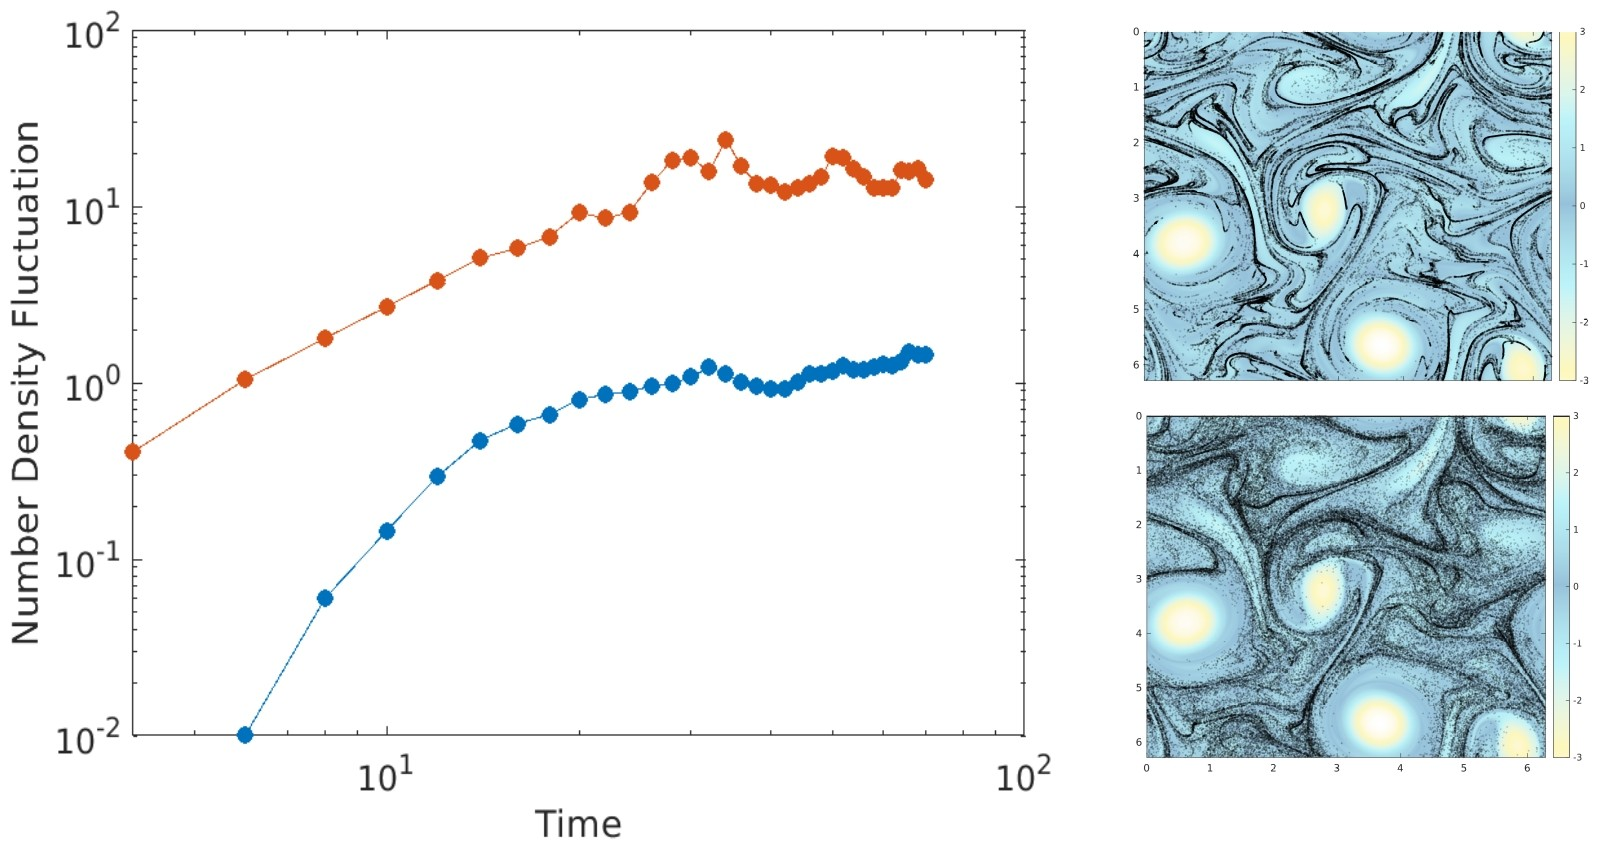
\includegraphics[width = 0.8 \linewidth]{./figures/active_caustics/density_fluctuation_measure.jpg}
%\hspace{0cm}\newline
\caption[Saturation of the number-density fluctuations in time]{\label{act-fig:3}\textbf{Number-density fluctuations:} The fluctuations saturate as a function of time as the particulate structure evolves from a uniformly random state to exhibiting caustics. Red and blue curves correspond to $l^2/\mathrm{w}_{0}^{2} = 2 \times 10^{3}$ and $l^{2}/\mathrm{w}_{0}^{2} = 0$ respectively. The activity $\beta/\kappa = 236$ in both cases. The top and bottom panels on the right correspond to the top and bottom curves on the left respectively. }
\end{center}
\end{figure}

\section{Active Preferred-length Dimer in a Point Vortex}
\label{act-ABPvortex}
The equations for an active dimer which has a preferred length are given by
\begin{align}
\dot{\mathbf{X}} & =  \vec{u} + \beta \mathbf{w}% \equiv \vect{v},   
\label{act-eqn:dimerX5s}\\
\dot{\mathbf{w}} & = \frac{1}{\tau_{\rm act}}\left(1 - \frac{|\mathbf{w}|^2}{\mathrm{w}_{0}^{2}} \right)   \mathbf{w} + (\alpha_{\rm act} \mathbf{S} + \mathbf{A})\cdot\mathbf{w} \nonumber \\ & - {l}^{2} \nabla^{2} \vec{u} \, %+ {\sqrt{2D} \over \tau_{\rm act}}\vec{\eta}(t)\label{act-eqn:dimerX6}.
+ \sqrt{2D_\eta}\vec{\eta}(t). \label{act-eqn:dimerX6s}%{+ {\bf f}(t)},\label{act-eqn:dimerX6s}
\end{align}
With $l = 0$ and $\vec{\eta} =0$,  \eqref{act-eqn:dimerX5s} and \eqref{act-eqn:dimerX6s} can be recast as
\begin{equation}
\frac{d \vec{v}}{dt} - \vec{v}\cdot\nabla \vec{u} = \,(\vec{u} - \vec{v}) \cdot \tilde{\tau}_{\rm act}^{-1}
\label{act-eqn:36}
\end{equation}
where $\tilde{\tau}_{\rm act}^{-1} \equiv \frac{\mathbb{I}}{\tau_{\rm act}} \left(\frac{||\vec{v}-\vec{u}||}{\beta^{2}} - 1 \right) - ( \alpha_{\rm act} \, \mathbf{S} + \mathbf{A} \,)$. The non-dimensional equations with $L = \sqrt{\tilde{\Gamma} \tau_{\rm act}}$ and $T = \tau_{\rm act}$, in cylindrical polar coordinates become
\begin{align}
\tilde{\beta}^2 \frac{d^{2} r}{dt^{2}} & = \tilde{\beta}^2 r \left( \frac{d\vartheta}{dt}\right)^{2} \nonumber \\
& + \frac{dr}{dt} \left\{ 2\frac{d\vartheta}{dt} -  \left( \frac{dr}{dt}\right)^{2} -r^{2} \left( \frac{d\vartheta}{dt}\right)^{2} + \tilde{\beta}^2 - \frac{1}{r^{2}} \right\} \nonumber \\
& + \frac{\tilde{\beta}^2 \alpha_{\rm act}}{ r^{3}}  - \frac{\tilde{\beta}^2 (1+\alpha_{\rm act})}{ r} \frac{d\vartheta}{dt},
\end{align}
\begin{align}
\tilde{\beta}^2 r \frac{d^{2} \vartheta}{dt^{2}} & = - 2 \tilde{\beta}^2 \frac{d\vartheta}{dt}\frac{d\vartheta}{dt}  + + \left( r \frac{d\vartheta}{dt} - \frac{1}{r} \right) \times \nonumber \\
& \left\{ 2\frac{d\vartheta}{dt} -  \left( \frac{dr}{dt}\right)^{2} -r^{2} \left( \frac{d\vartheta}{dt}\right)^{2} + \tilde{\beta}^2 - \frac{1}{r^{2}} \right\} \nonumber \\
& - \frac{\tilde{\beta}^2 (1+\alpha_{\rm act})}{ r^{2}} \frac{dr}{dt},
\end{align}

where $\tilde{\beta} \equiv \beta \sqrt{\tau_{\rm act}/{\tilde{\Gamma}}}$ is the non-dimensional motility. Writing $v_{r} = dr/dt$ and $\dot{\vartheta} = d\vartheta/dt$, these may be recast more compactly as
\begin{align}
%\label{act-total_sol}
\frac{dr}{dt} & = v_{r}, \label{act-abp_r}\\
\tilde{\beta}^2 \frac{dv_{r}}{dt} &= \tilde{\beta}^2 r\dot{\vartheta}^{2}  + v_{r} \left\{ 2\dot{\vartheta} -  {v_{r}}^{2} -r^{2} {\dot{\vartheta}}^{2} + \tilde{\beta}^2 - \frac{1}{r^{2}} \right\} \nonumber \\
& +  \frac{\tilde{\beta}^2 \alpha_{\rm act}}{r^{3}} - \frac{\tilde{\beta}^2 (1+\alpha_{\rm act})\,\dot{\vartheta}}{r}, \label{act-abp_v}\\
\tilde{\beta}^2\ddot{\vartheta} & = - \frac{2 \tilde{\beta}^2\, v_{r} \, \dot{\vartheta}}{r}  \nonumber \\
& + \left( \dot{\vartheta} - \frac{1}{r^{2}} \right) \left\{ 2\dot{\vartheta} -  {v_{r}}^{2} -r^{2} {\dot{\vartheta}}^{2} + \tilde{\beta}^2 - \frac{1}{r^{2}} \right\} \nonumber \\
& - \frac{\tilde{\beta}^2(1+\alpha_{\rm act})\, v_{r}}{r^{3}} \label{act-abp_omega}.
\end{align}

By calculating the divergence of crossing time, for a fixed $\tilde{\beta} =1.0$, we get the caustics phase in the $r-\alpha_{\rm act}$ plane, similar to the hookean case. We find that rigid spheroidal microswimmers  \cite{Stark2012, Stark2016} in vortical flow also display caustics, which we do not explore here.

\begin{figure}[t]
\begin{center}
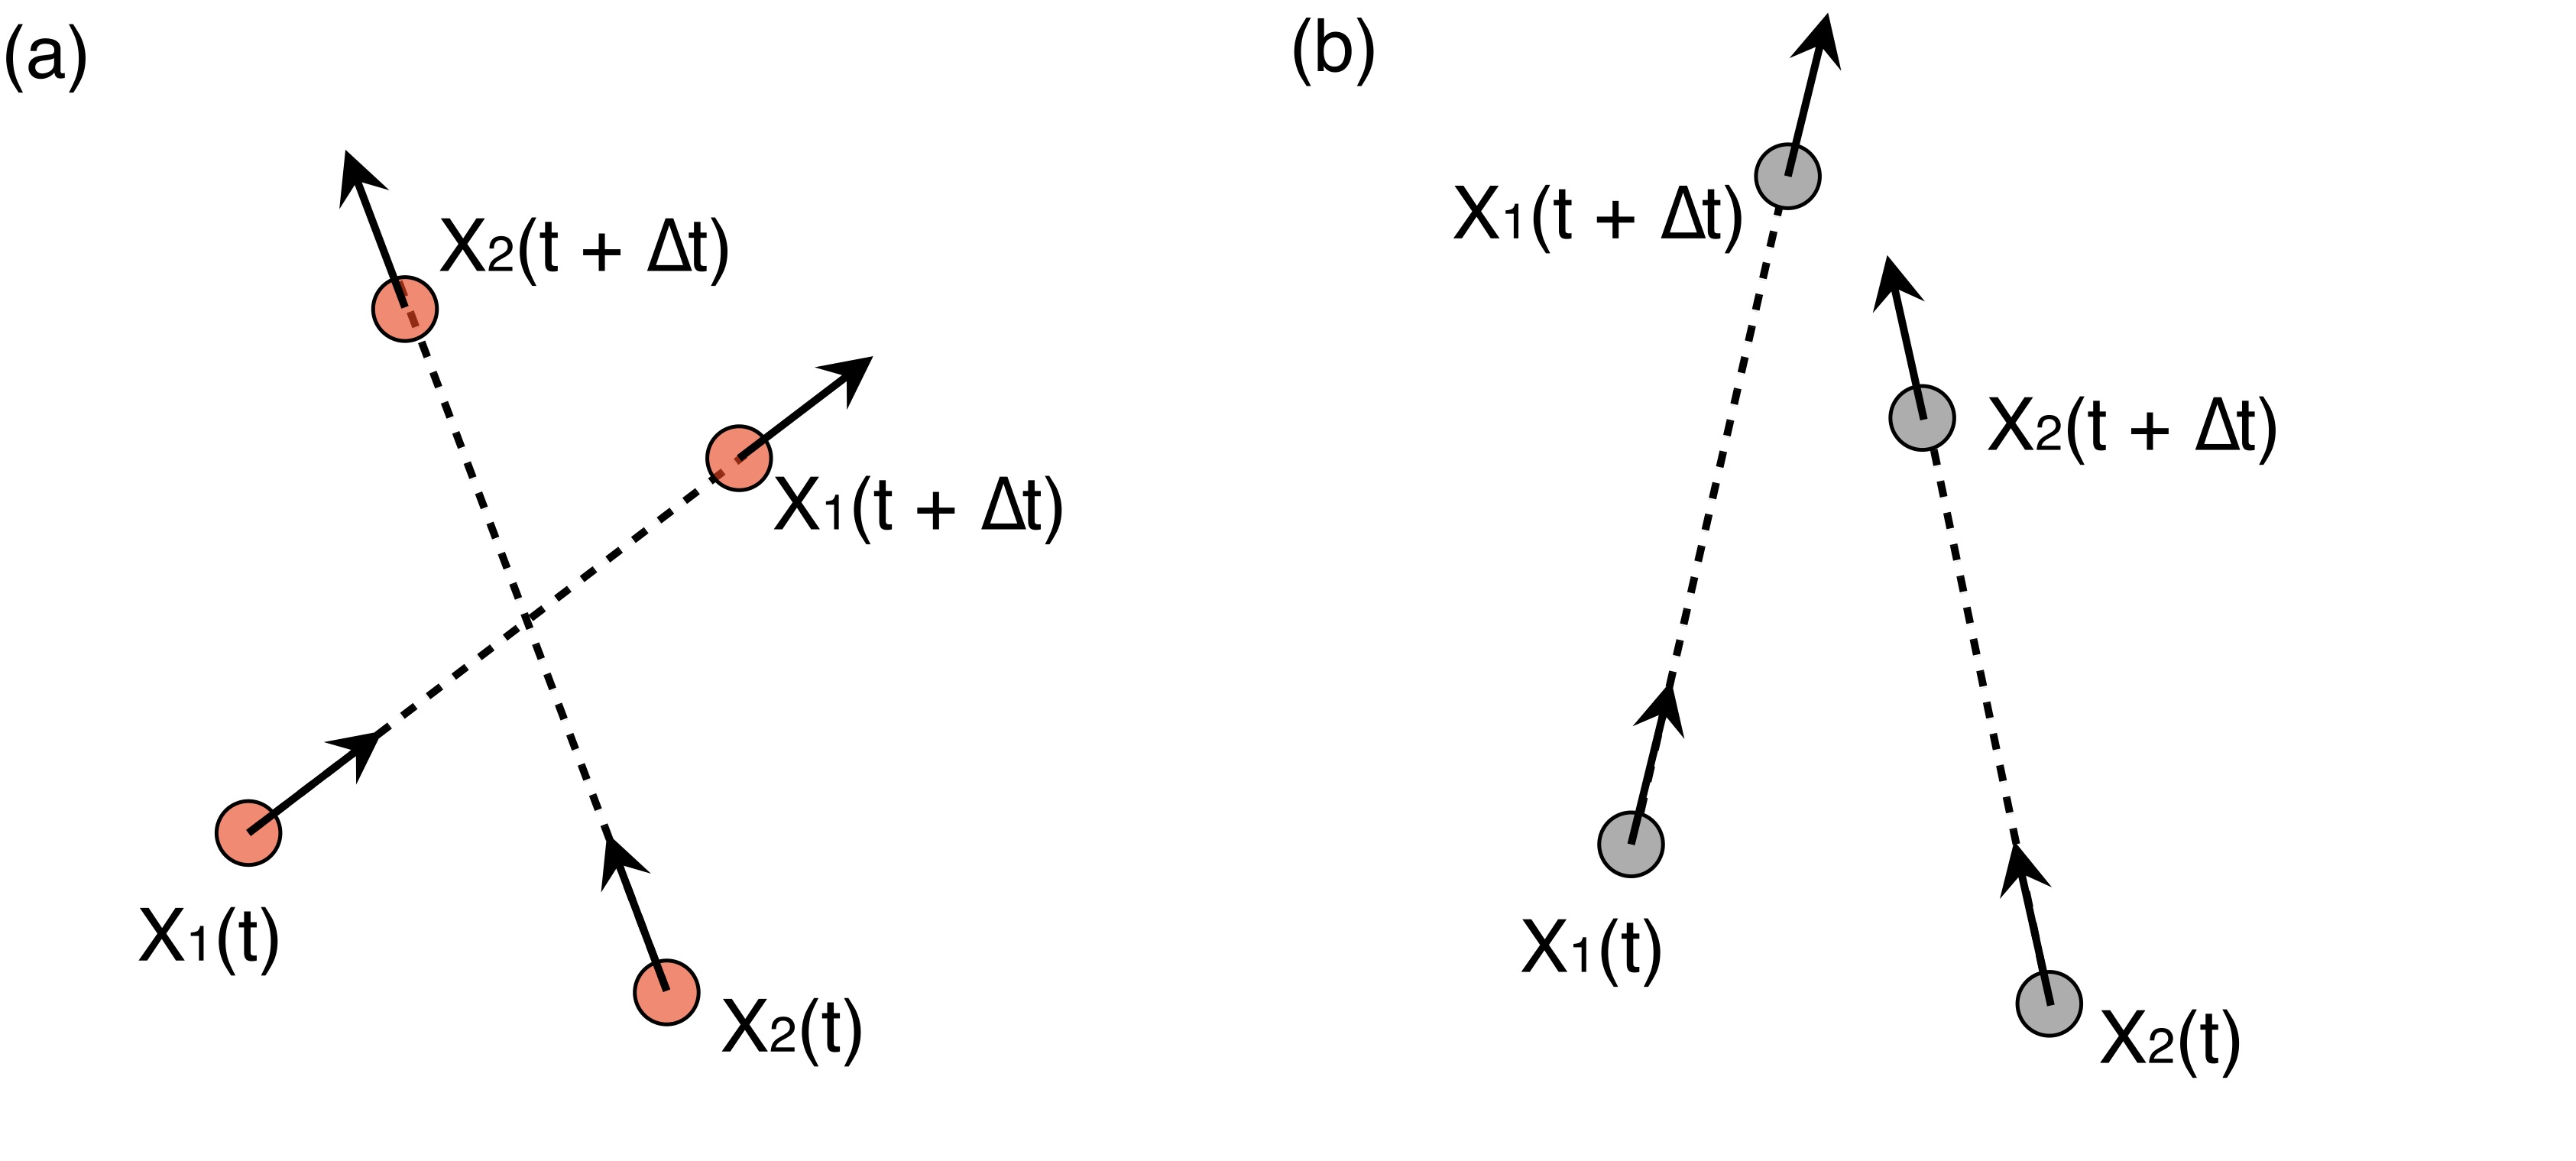
\includegraphics[width = 0.7 \linewidth]{./figures/active_caustics/collision_schematic.jpeg}
%\hspace{0cm}\newline
\caption[Schematic of colliding and non-colliding particle pairs]{\label{act-fig:collision}\textbf{Collisions:} A schematic of (a) colliding (red) and (b) non-colliding (grey) pairs of particles, where the intersection of paths within the numerical time step $\Delta t$ marks the collision event.}
\end{center}
\end{figure}
\section{Number density fluctuation, clustering and collisions}
\label{act-denflu}
Local number density fluctuations can be used as a statistical measure for the intensity of caustic-induced clustering. The space is numerically discretized into $N_{\rm bin} \times N_{\rm bin}$ cells such that there is on an average 1 particle per cell in the initial uniformaly random state
\begin{equation}
    {\Delta \rho_{ij}}^{2} = \frac{1}{N_{\rm bin}^2}\sum_{i,j} (\rho_{ij} - 1)^{2}.
\end{equation}
Here, $i,j$ are the cell index corresponding to a given spatial location. The initial state itself contributes a residual density fluctuation, which we subtract to obtain purely caustic-induced clustering. 
To measure collisions, we find pairs of particles whose trajectories intersect within the numerical time step $\Delta t = 10^{-3}$, as shown in \ref{act-fig:collision}. Such particles are colored red in Supplementary Video 5; where we one finds that the regions with high number-density coincide with the crossing of particle trajectories.

\chapter{Lucky drops grow bigger: but luckier drops get less lucky}

\section{Polydisperse droplet growth in the outer region of point vortex}
Despite continuously centrifuging, monodisperse inertial particles do not form caustics in the outer region of the point vortex. The outer region, starts around $\text{O}(\sqrt{\Gamma\tau_p/2\pi})$ distance from the vortex origin,  gives minimal radial acceleration to the inertial particles. However, particles of different sizes can still collide because they differ in centrifugation velocity. Here we study that growth rate of centrifuging polydisperse particles. Like in the text, we consider two kinds of particles, a continuum of small particles, and a single big drop. We wish to obtain growth rate of the big drop as a function of time in these regions.

\subsubsection{Number density as a function of the radius}
The first step is to calculate the number density of small droplets in terms the distance from the origin. Given the particles are continuously centrifuging it should also be a function of time. For the remainder of this section, we will ignore the subscript $s$ on quantities. The number density field obeys
\begin{align}
% \label{}
\begin{split}
    \frac{d n }{d t} = - n \div{\vec{v}}.
\end{split}
\end{align}
The radial velocity in the outer region of a particle with Stokes number $St$ is given by
\begin{align}
% \label{}
\begin{split}
    \vec{v}(t) = \frac{St}{r(t)^3}\vec{e}_r + \frac{\vec{e}_\vartheta}{r(t)},\quad \text{with } r(t) = (r^4(0) + St~t)^{\frac14},
\end{split}
\end{align}
where we have adopted the cylindrical coordinates $(r,\vartheta,z)$ and assumed that particle started from the same velocity as the background fluid. This makes $\div{\vec{v}} = -2 St/r^4$. Putting this back in the continuity equation, we get
\begin{align}
% \label{}
\begin{split}
    d\left[ \ln n(t) \right] = 2 \frac{St~ dt}{r^4(t)}.
\end{split}
\end{align}
Integrating the outer solution readily gives
\begin{align}
% \label{}
\begin{split}
    \frac{n}{n(0)} = \left[\frac{r^4(0) + St ~ t}{r^4(0)}\right]^2 \quad \implies n(t) = n(0)\left(\frac{r(t)}{r(0)}\right)^8.
\end{split}
\end{align}
Thus, we have $n(r)$ however, one should remember that $n(0)$ and $r(0)$ are the Lagrangian initial condition, not the Eulerian one.
\subsection{Collisional growth}\textcolor{red}{rewrite}
Now that we know $n(r)$, we can directly compute the growth rate of the big droplets from Eq. \eqref{lucky-3Deqns}. Plugging in the values, it reads
\begin{align}
% \label{}
\begin{split}
    \dot{St}_b &= \sqrt{\frac{St_b \rho Re}{18}} \left( 1 + \sqrt{\frac{St_s}{St_b}} \right)^2 c_s(r_b) \left|\dot{r}_b - \frac{St_s}{r_b^3(t)}\right| \\
    \ddot{r}_b - \frac{1}{r_b^3}&=  \sqrt{\frac{\rho Re}{8St_b}}\left( 1 + \sqrt{\frac{St_s}{St_b}} \right)^2 c_s(r_b) ~ \left|\dot{r}_b - \frac{St_s}{r_b^3(t)}\right|\left(  \frac{St_s}{r_b^3(t)}-\dot{r}_b\right)+ \frac{\left(\dot{r}_b\right)}{St_b} \ ,
\end{split}
\end{align}
where $c_s(r_b) = c_s(0,r_s(0))\left( r_b^8/r_s(0)^8 \right)$, such that $r_s(t) = r_b$. Note if the lucky droplets weren't colliding with the smaller ones, we could have neglected $\ddot{r}_b$ and obtained a straightforward expression for $\dot{r}_b$. But in presence of collision, we need to rederive the outer solution of $r_b(t)$, and $St_b(t)$.
\section{Number density field?}

Turns out in $3$D, the number density field does not behave as well as in $2$D. Fig. \ref{lucky-n-snp} shows the difference in physical structure, and Fig. \ref{lucky-n-spectra-slope}(right) compares the field spectra with the Lagrangian spectra.
\begin{figure}
	\begin{center}
		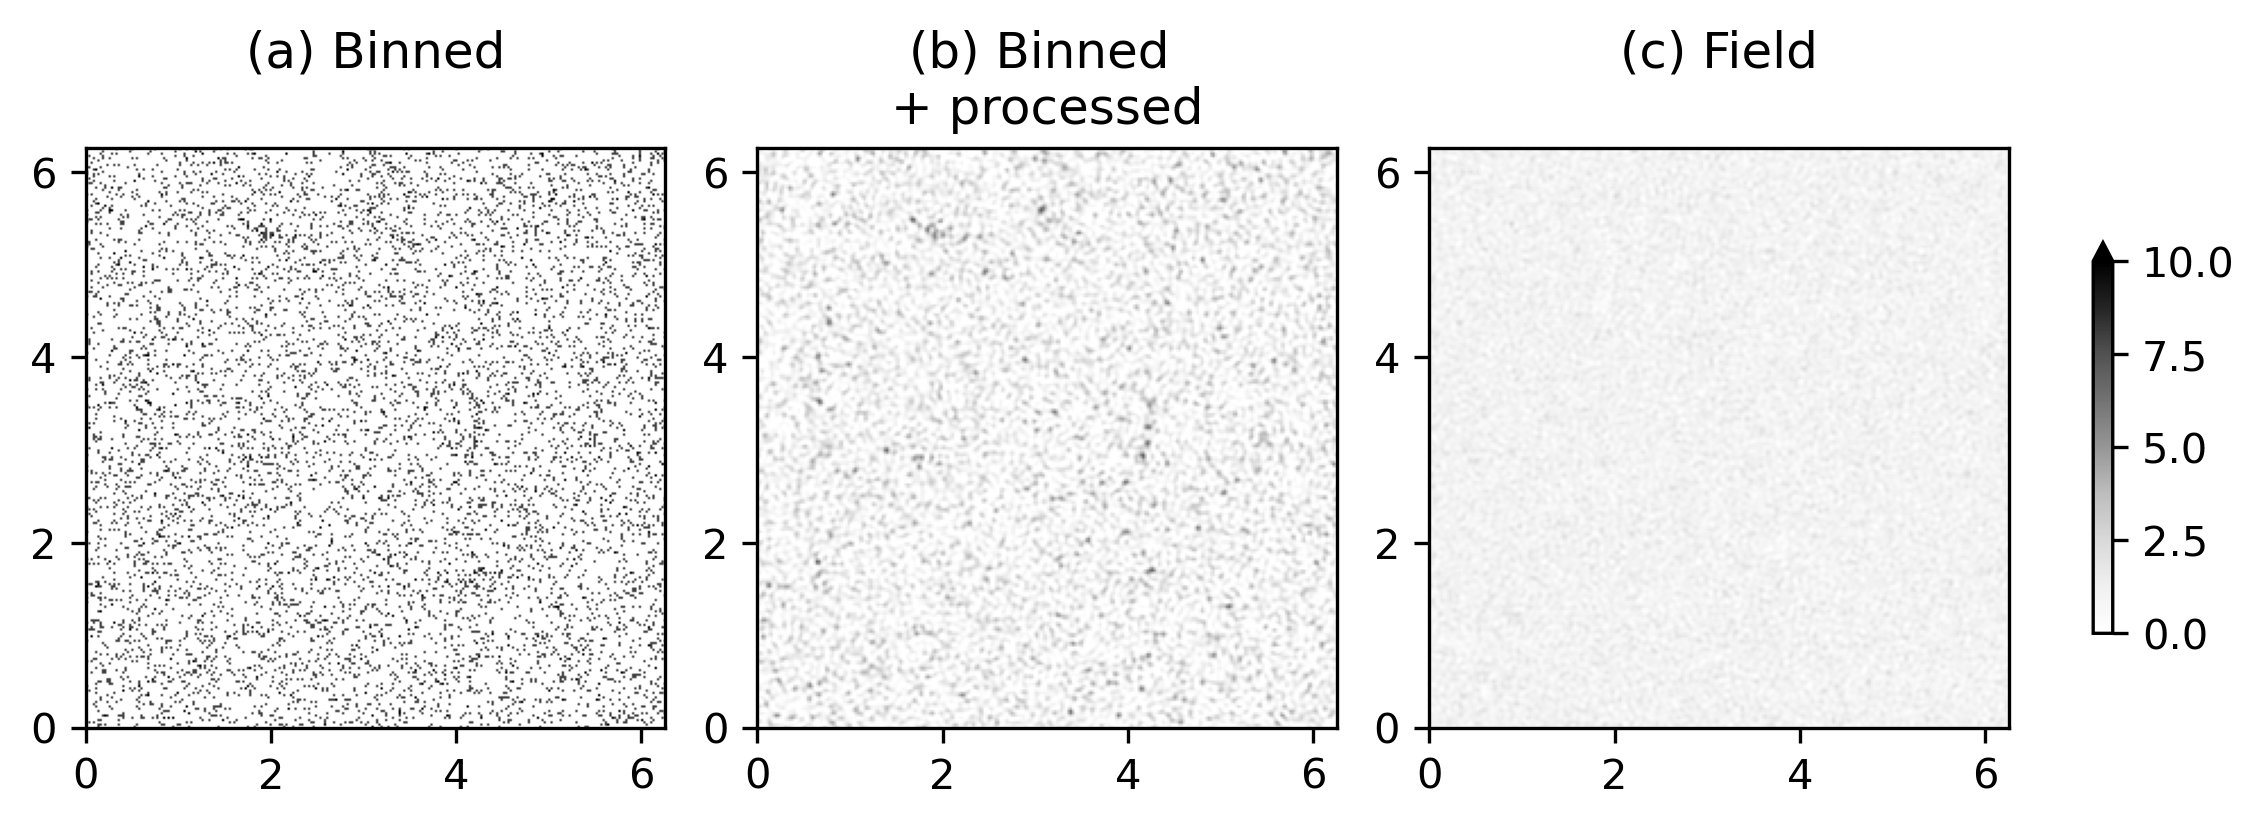
\includegraphics[width=\linewidth]{./figures/polydisperse/n-snapshot-st-0.001.png}
	\end{center}
\caption[Snapshot of the number density field]{Y-Z snapshot of the number density field for the cases. $St = 0.001$}
\label{lucky-n-snp}
\end{figure}

There are also differences when one directly bins or smears the distribution using a Dirac-delta function approximated over the grid-points. In Fig. \ref{lucky-n-spectra-slope}(left) are the two spectra for the binned and the Delta-function smeared number density. We see that the small scale large $k$ magnitudes differ. This happens for two reasons. First, the binned version is not inherently periodic, while the Delta-function smeared one is. Secondly, the binned one is much more susceptible to particle position, and does not take into account the position of each particle within the grid causing larger fluctuations between grid points.
\begin{figure}
	\begin{center}
		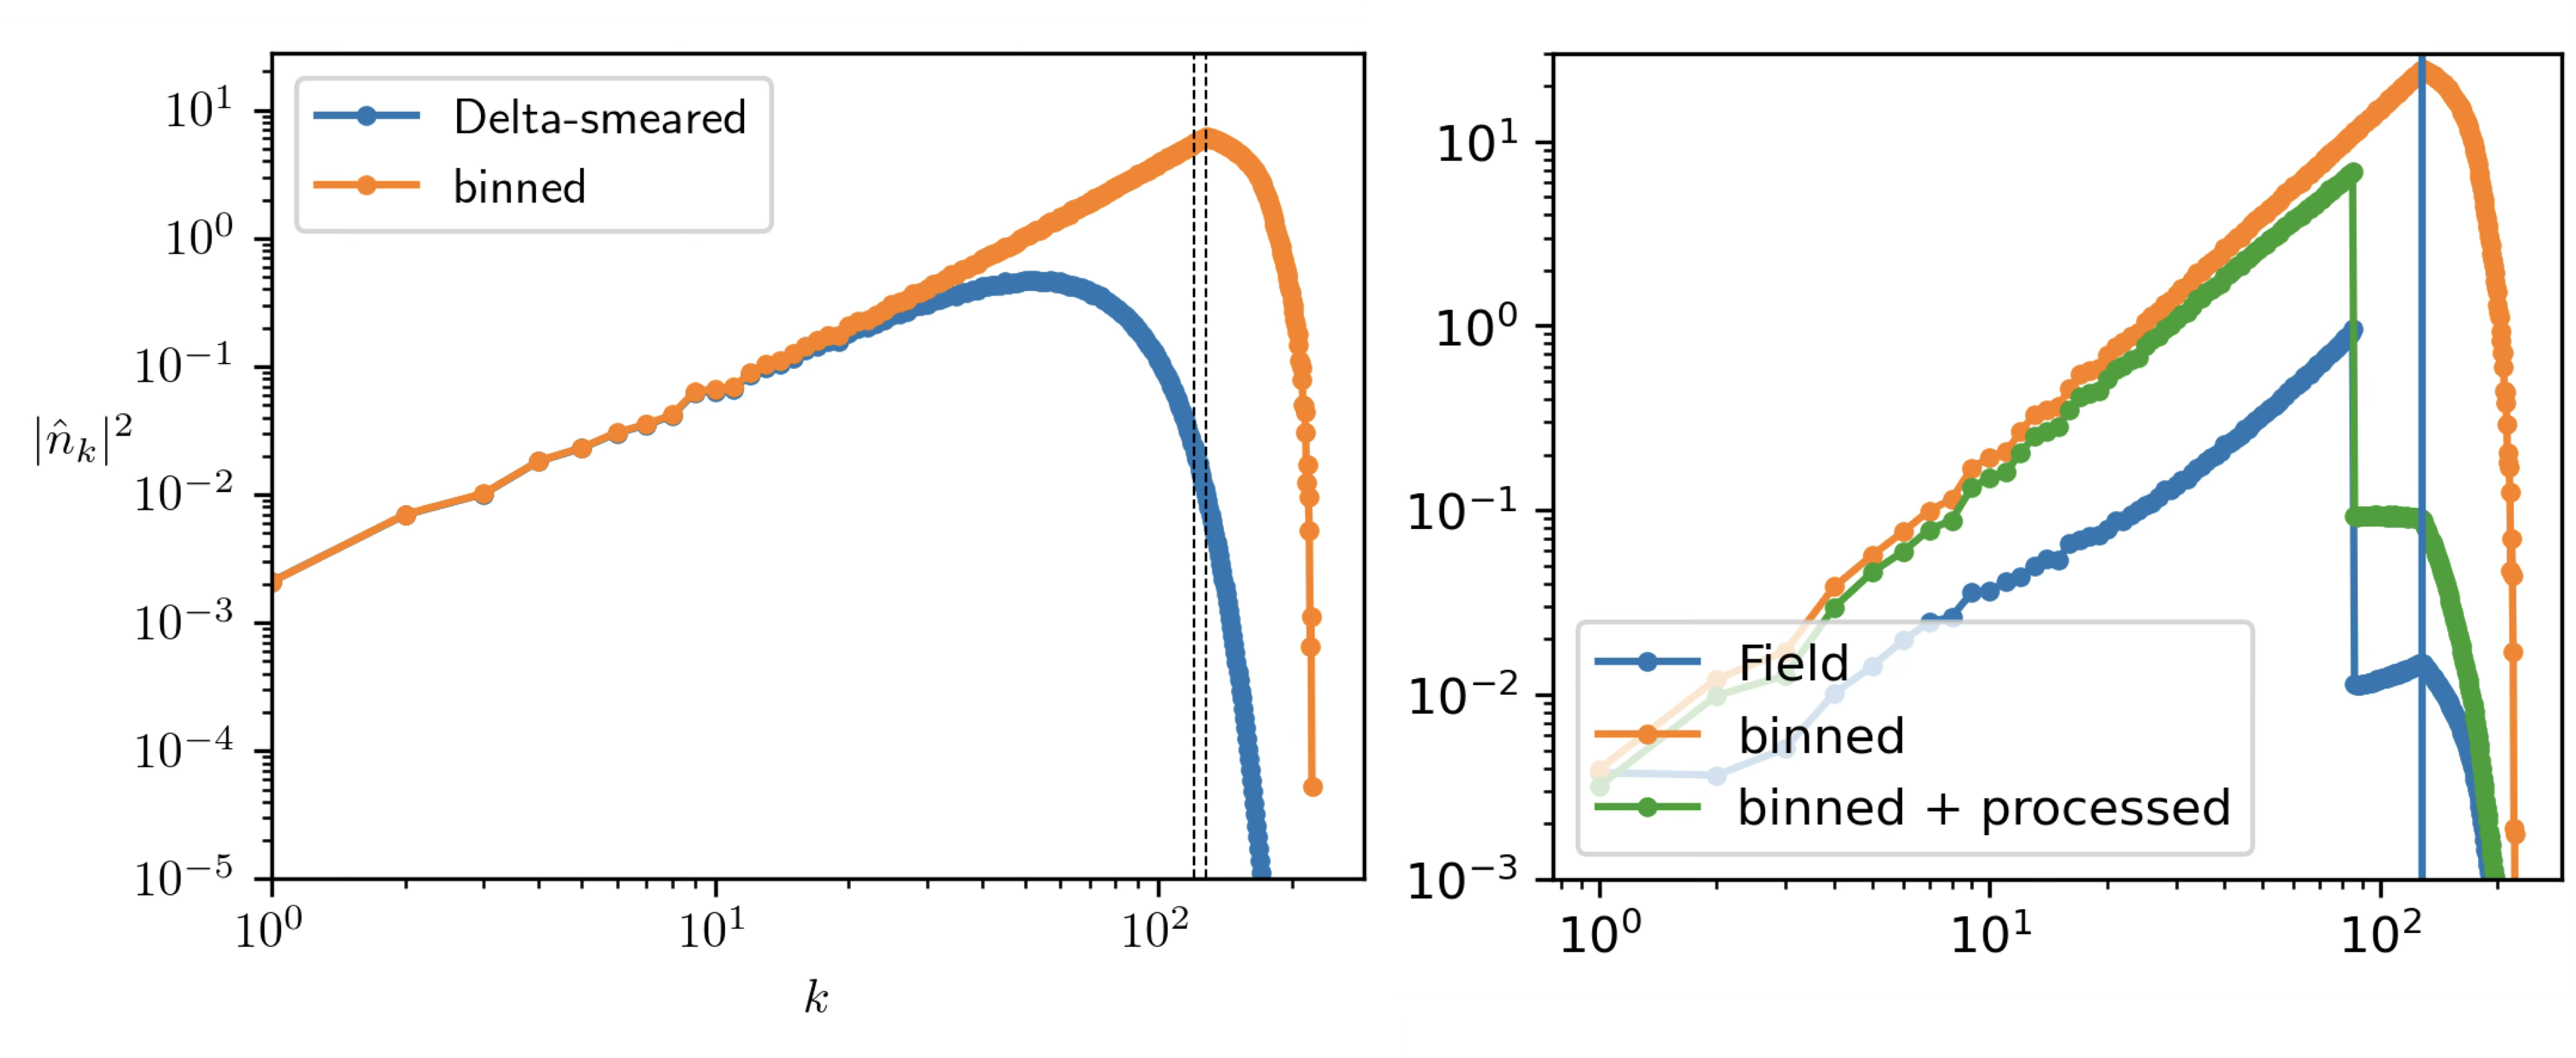
\includegraphics[width=\linewidth]{./figures/polydisperse/n-spectra-slope.png}
	\end{center}
\caption[Number density spectra from smearing, binning, and field equations]{(left) Delta-smeared v binned spectra of the number density. (right) Comparing spectra from lagrangian evolution, then binning v evolving the field equations of the $n$ field.}
\label{lucky-n-spectra-slope}
\end{figure}
However, such small difference in large $k$ amplitude considerably changes the structure of the field, which Fig. \ref{lucky-struc-binned-v-smeared} clearly shows in its difference in the limits of the colorbar.
\begin{figure}
	\begin{center}
		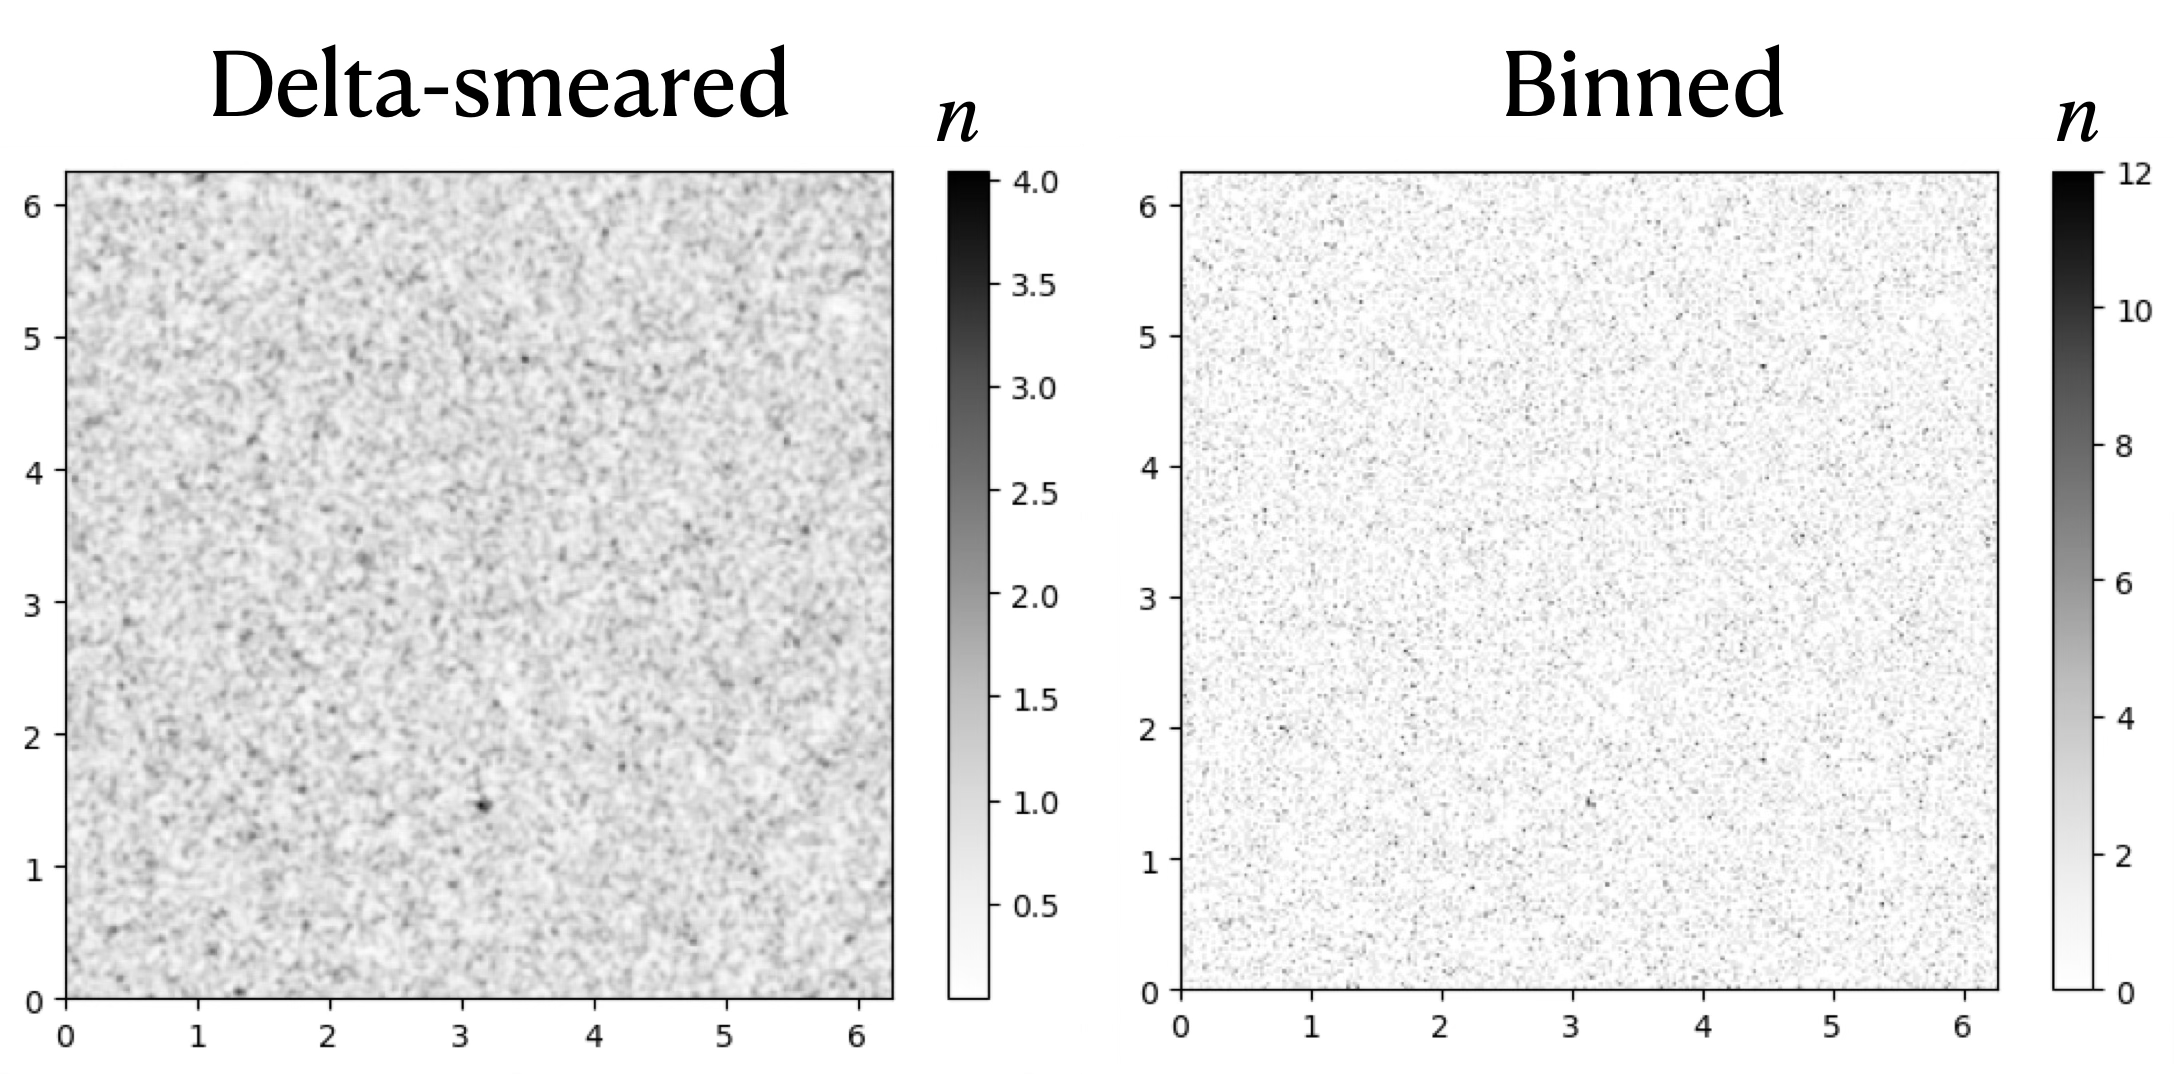
\includegraphics[width=\linewidth]{./figures/polydisperse/binned-v-smeared-comp.png}
	\end{center}
\caption[Number density structure from smearing compared with binning]{Physical structure of the $n$ field compared between smearing delta-function and naive binning. The particle follows slow-manifold approximation with $St = 0.001$.}
\label{lucky-struc-binned-v-smeared}
\end{figure}


\section{Correlation of the local number density across Stokes number}
\begin{figure}
	\begin{center}
		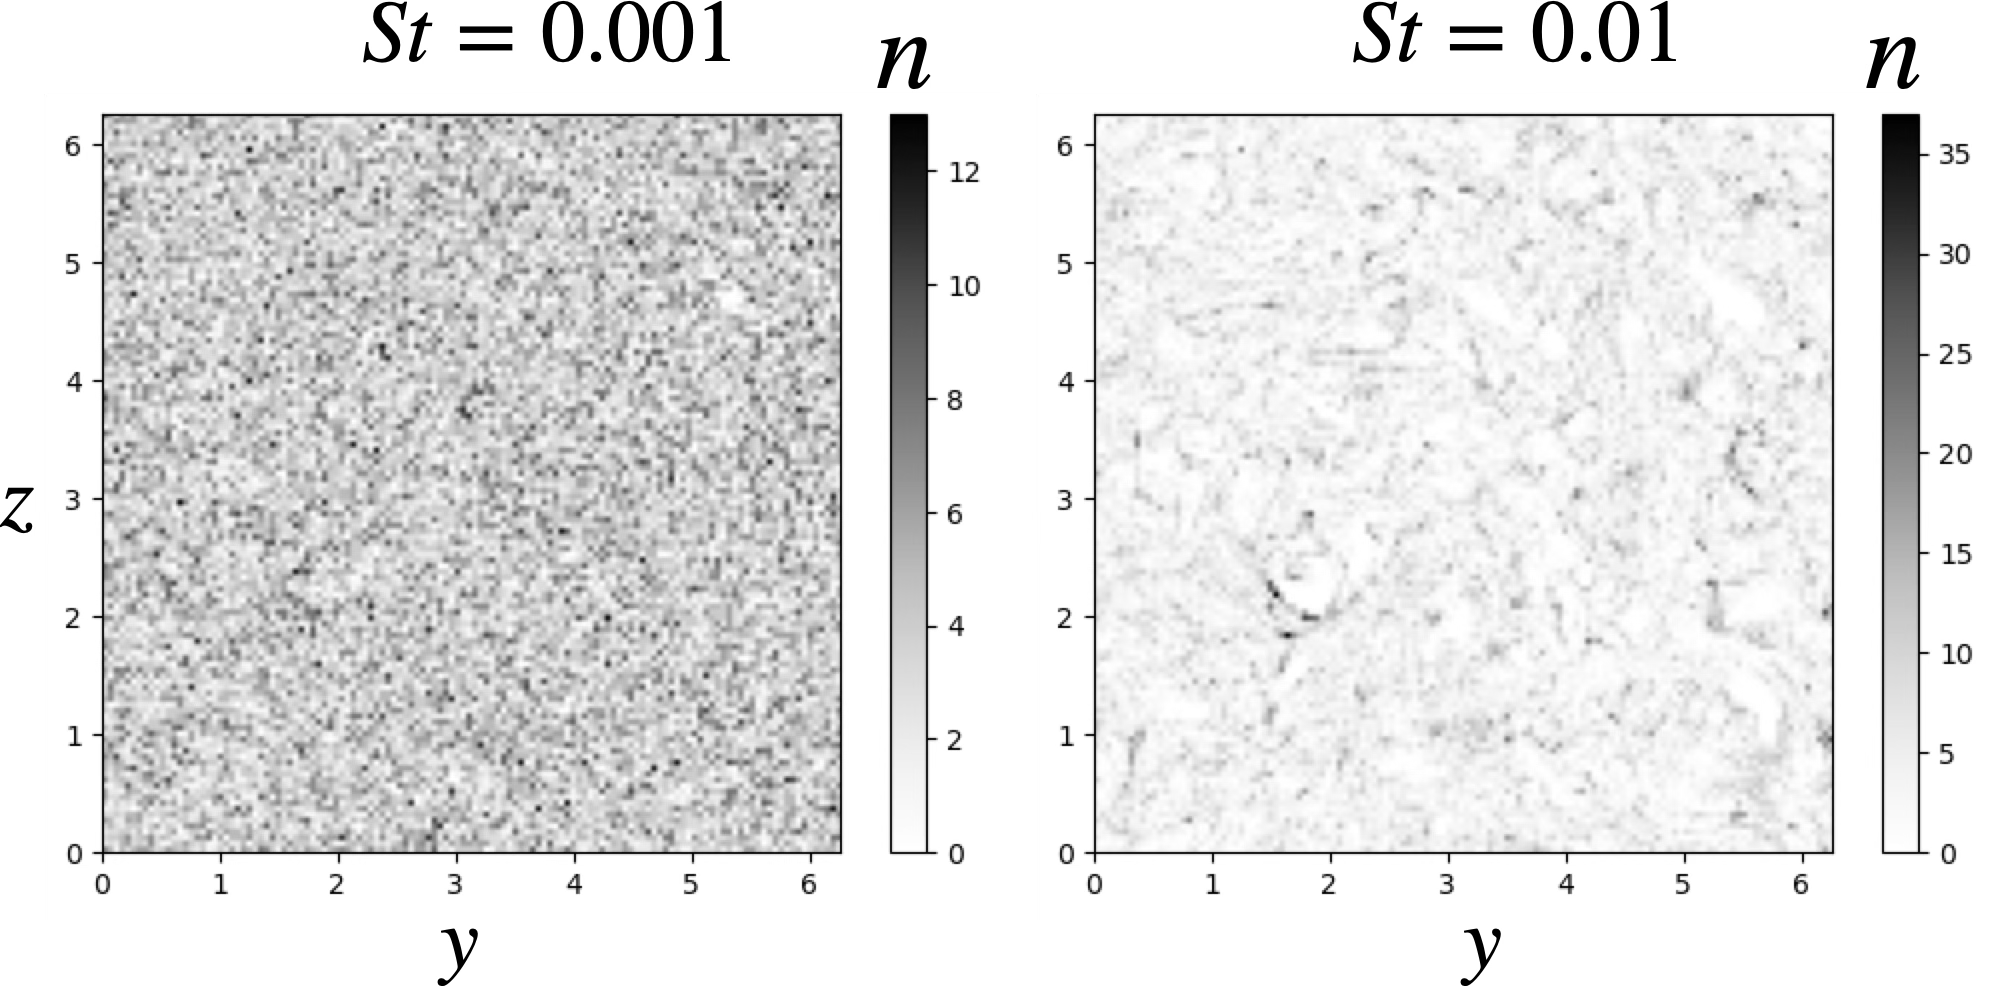
\includegraphics[width=\linewidth]{./figures/polydisperse/dist-nbin-128.png}
	\end{center}
\caption[Binned number density distribution for $128^3$ bins]{Same as Fig. \ref{lucky-nbin-dist-256} but the number of bins is $128^3$.}
\label{lucky-nbin-dist-128}
\end{figure}

\begin{figure}
	\begin{center}
		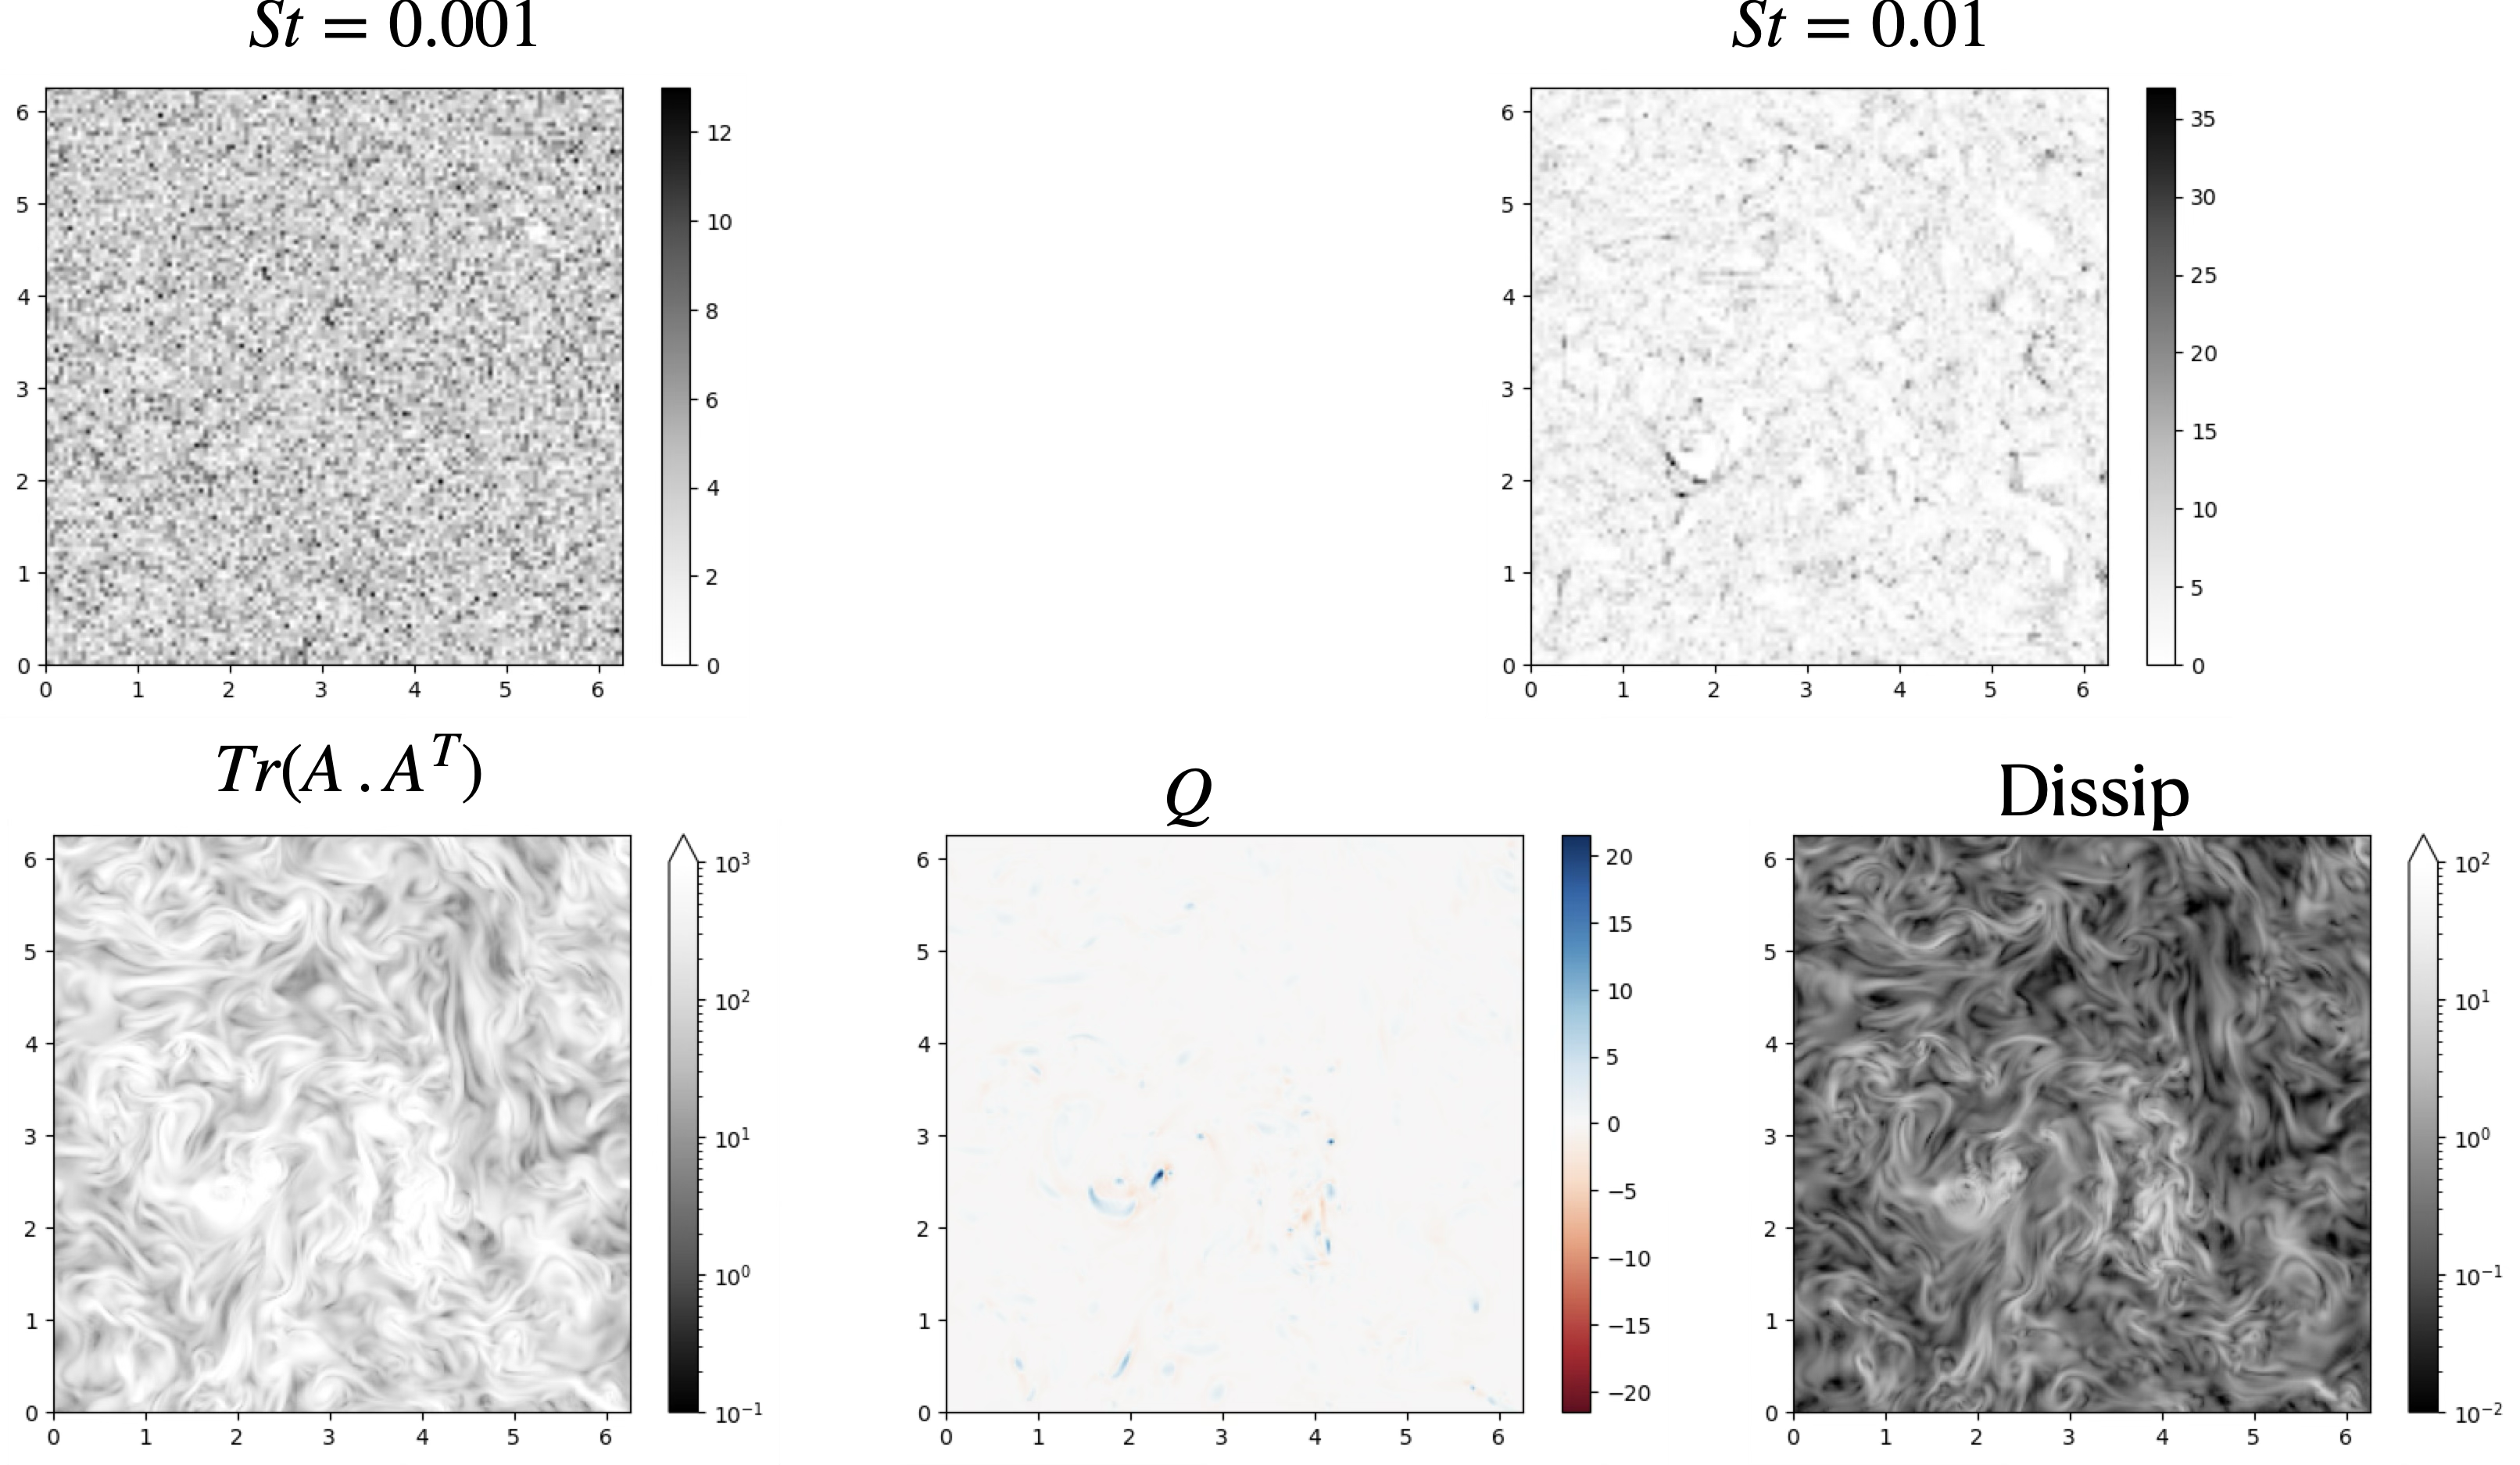
\includegraphics[width=\linewidth]{./figures/polydisperse/grad-corr.png}
	\end{center}
\caption[Binned number density with background gradients]{Binned number density with background gradients. Nbins  = $128^3$ }
\label{lucky-grad-corr}
\end{figure}
\subsection{Effect of correlated collisions}
What if the number density was spatially correlated? Well we could investigate with $St = 0.01$ and re-plot Fig. \ref{lucky-3d-grwth}. But now we have a cheap stochastic way to evolve, generating $n_s$ form a random distribution. So, if we can generate a spatially correlated number density, we are good. Turns out we can. For example drawing from a distribution
\begin{align}
\label{lucky-gen-pois}
\begin{split}
    P_{\vec{x}}(n) = \frac{\lambda(\vec{x})^n}{n!}e^{-\lambda(\vec{x})},\quad \quad \text{with } \lambda(x) = \bar{\lambda} \frac{\partial_j u_i \partial_j u_i}{\langle \partial_j u_i \partial_j u_i \rangle_x} ,
\end{split}
\end{align}
where $\bar{\lambda}$ is the average number of particles per unit grid. Such a distribution looks like as given below.
\begin{figure}
	\begin{center}
		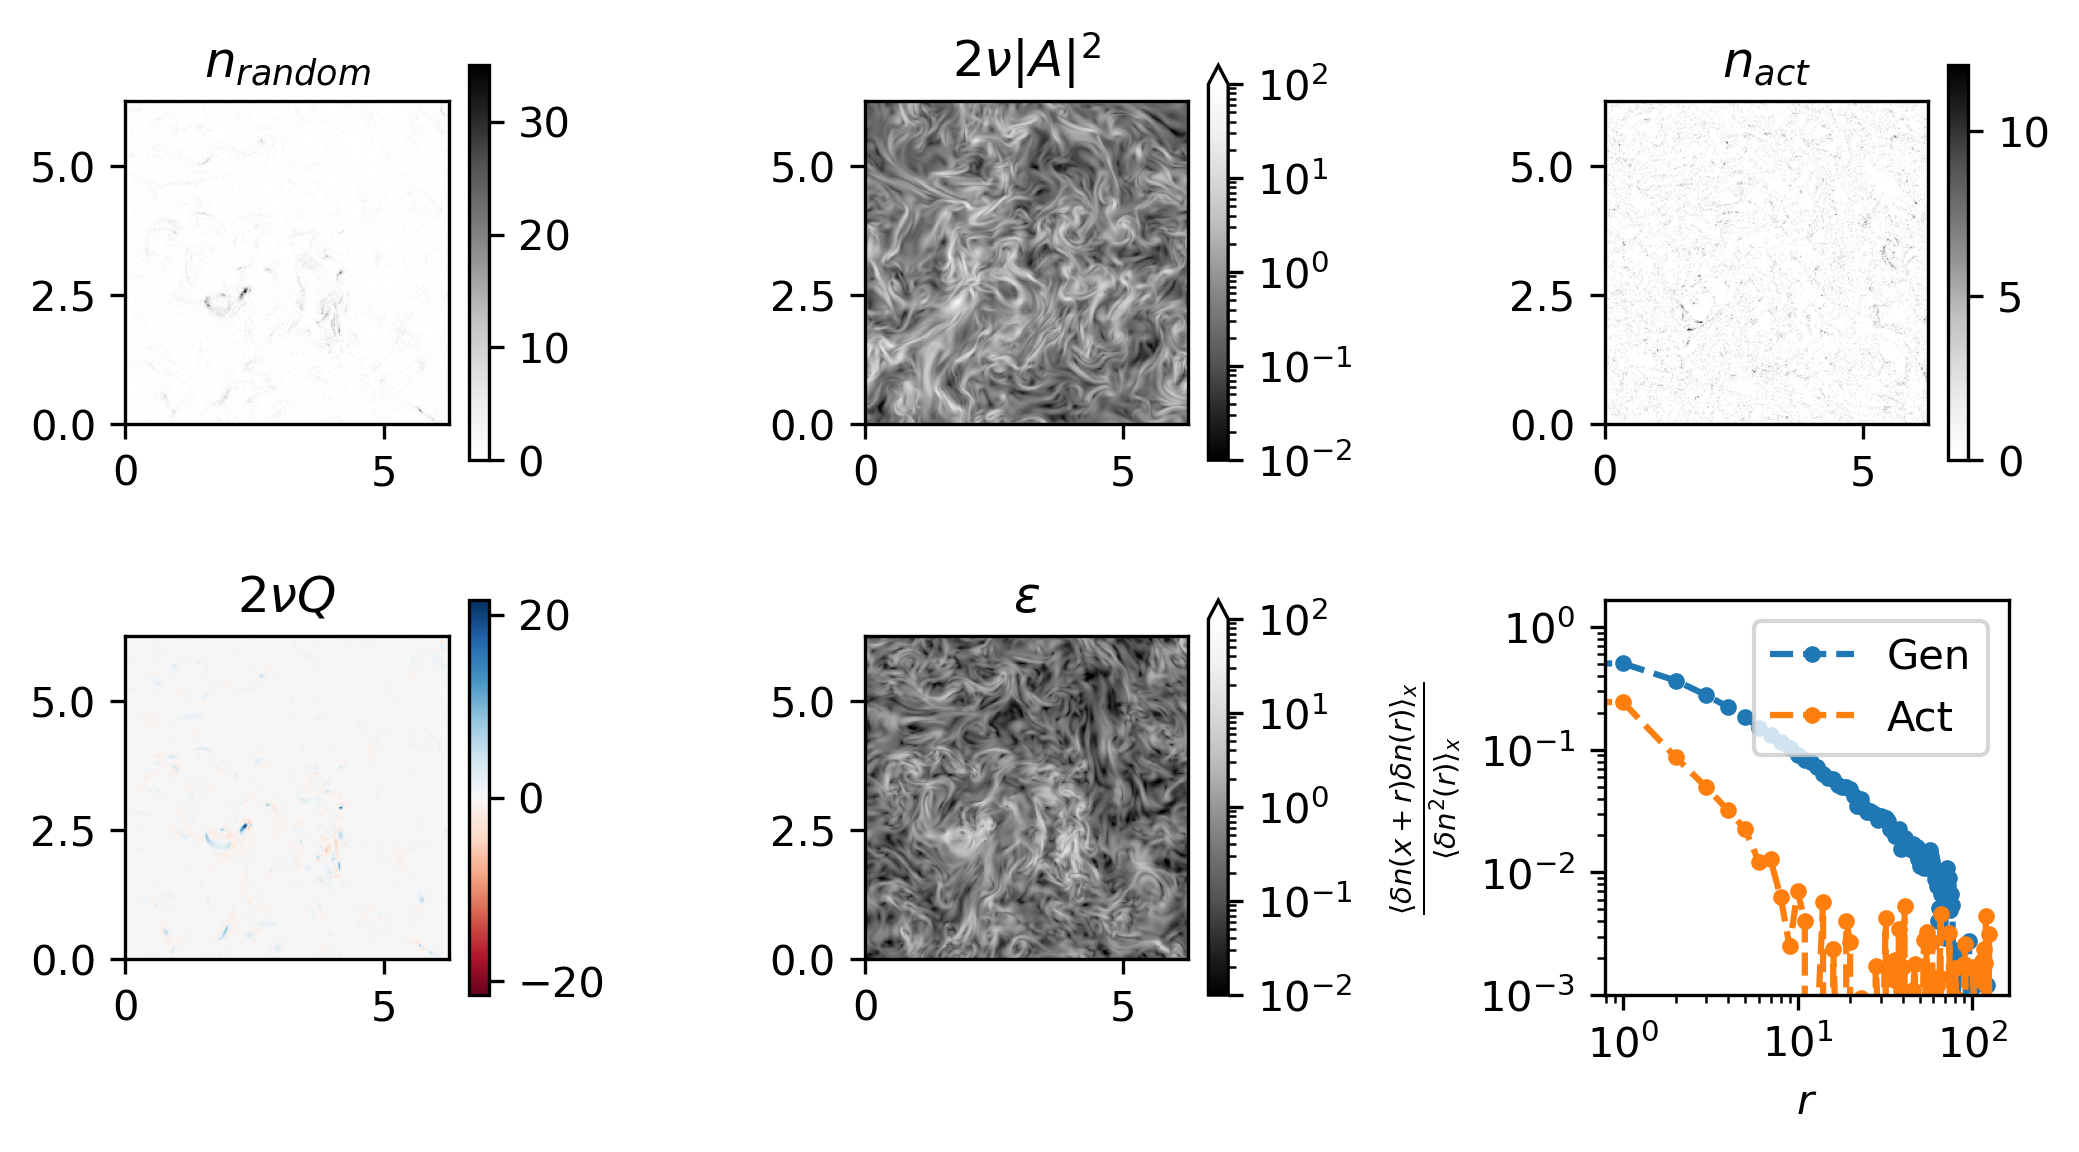
\includegraphics[width=\linewidth]{./figures/polydisperse/gen-corr.png}
	\end{center}
\caption[Correlated distribution compared with slow-manifold particles]{Comparing correlated distribution generated from Eq. \eqref{lucky-gen-pois} with field gradients and actual distribution of $St = 0.01$ slow manifold particles. }
\label{}
\end{figure}


\section{Relating the simulation numbers with physical parameters }\label{lucky-sim-relate}
For numerical simulations, we do not directly put in the cloud parameters listed in table \ref{lucky-cloud-vals}. There, the box-size is fixed $L = 2\pi$, and so is the power input which equals to the time average dissipation $\bar{\epsilon}$. Although we can match the viscosity and the $\bar{\epsilon}$ values with the ones listed in table \ref{lucky-cloud-vals}, we do a simpler calculation. Artificially setting any viscosity gives us a numerical Kolmogorov length scale at the stationary state $\eta_{num} = (\nu_{num}^3/\epsilon_{num})^{1/4}$. Similarly, the Kolmogorov timescale is also set $\tau_{\eta_{num}} = \sqrt{\nu_{num}/\epsilon_{num}}$. Matching these with the values listed in table \ref{lucky-cloud-vals} gives us our length and time scales. Therefore, in the dimensional units, our box size, and timescale will be
\begin{align}
% \label{}
\begin{split}
    L_{box} = 2\pi\frac{\eta}{\eta_{num}}\quad ;\quad T = \frac{\tau_\eta}{\tau_{\eta_{num}}}.
\end{split}
\end{align}



\section{Relating the weird definition of number density and the number of particles in a given volume}

The field number density plotted is normalized such that its mean is $1$. But it is wise to relate the actual number density whose average gives the average number of particles in unit volume. Thus, the number density plotted is the actual number density divided by the number of particles in unit volume given by $N_V$.

From the length and timescales used in Appendix \ref{lucky-sim-relate}, the number of particles per unit volume in the simulation unit becomes
\begin{align}
\label{}
\begin{split}
    N_V = \frac{6c_s}{\pi}\frac{\eta^3}{d_s^3 \eta_{num}^3},
\end{split}
\end{align}
where $c_s$, and $d_s$ are the volume fraction and diameter of the small particles listed in table \ref{lucky-cloud-vals}.


\section{Stochastic collision in simulation units}
In the stochastic process, this is how the mass of the large particles are evolved.
\begin{figure}[h]
\centering
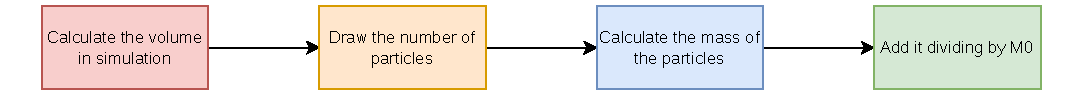
\includegraphics[width = \linewidth]{./figures/polydisperse/stochastic-collision.pdf}
\caption[Flowchart of stochastic collisions of big droplets]{Flowchart of stochastic collisions of big particles.}
\end{figure}
\section{Conversion between number density, number density used in code and number of particles}

The number density evolved in the code, $\tilde{n}_s$ is scaled such that its initial mean is 1. Thus, $\tilde{n}_s$ relates to the actual number density by $\tilde{n}_s= n_s\times (2\pi)^3/ N_s(0)$, where $N_s(0)$ is the initial number of small particles in  the domain. Lucky droplets would deplete this number, but the normalization stays same. The mean of $\tilde{n}_s$ decreases below $1$ with time. Now from a given initial mass fraction $M_s(0) = 7.2 \times 10^{-4}$, and given Stokes number, $St= 10^{-3}$, one needs to calculate $N_s(0)$. Table \ref{lucky-cloud-vals} tells us that this mass fraction is equivalent to having $10^{11}$ 2.7$\mu$m initial tiny droplets. To get the total number of particles in a given volume, we have to consider
\begin{align}
% \label{}
\begin{split}
    St &= \frac{\tau_p}{\tau_f} = \frac{1}{18} \rho \frac{d_s^2}{\eta^2} \\
    \implies  d_s&= \eta\sqrt{\frac{18 St}{\rho}}.
\end{split}
\end{align}
With this, $N_s(0)$ in a given domain $L$ is
\begin{align}
% \label{}
\begin{split}
    N_s(0) = \frac{6 M_s(0)L^3}{\rho \pi d_s^3}.
\end{split}
\end{align}

The maximum realistic value number density field can achieve in resolution of $\Delta x \Delta y \Delta z$ is
\begin{align}
% \label{}
\begin{split}
    n_s(t)|_{\text{max}} = \frac{N_s(t)}{\Delta x \Delta y \Delta z} = \mean{n_s(t)}N_g^3.
\end{split}
\end{align}
Similarly, the maximum value of $\tilde{n}_s(t) = \mean{\tilde{n}_s(t)}N_g^3. $

\section{Alternatives to clipping and rescaling the number density}\label{clip-alt}
Clipping the negative values to zero in the spectral evolution of the number density in Eqs. \eqref{lucky-3Deqns} and \eqref{lucky-2Deqns} is artificial. So is the rescaling to keep the mean zero. An alternative to keep the number density positive at all times would be to evolve the \texttt{log} of the number density, $g = \log(n_s)$. Without sinks and sources, it obeys
\begin{align}
\label{lucky-log-cont}
\begin{split}
    \partial_t g + v_s\cdot\grad{g} = - \div{v_s}.
\end{split}
\end{align}
The output of such evolution ensures that $n_s\geq 0$. However, there are two more problems with this method. First, values can go to $\pm \infty$ which a spectral code will then spread to everywhere. The fix is to set a lower limit (corresponding to machine precision in $n_s$) and a upper limit (corresponding to the maximum number of particles in a cell) of $g$ in the simulation. One can then rescale the entire $g$ to preserve the mean like before.

The second problem is more severe. Positive errors in $g$ gets exponentiated in $n_s$. Thus, the field $n_s$ may be wildly wrong. Indeed, this happens, as one can see in Fig. \ref{lucky-log_comp}. Comparing to the $n_s$ fields evolved with clipping and rescaling, it produces fluctuations in orders of magnitude more.
% \begin{figure}
% 	\begin{center}
% 		\includegraphics[width=\linewidth]{plots/log_comp.png}
% 	\end{center}
% \caption{Comparing fluctuations in of evolution of $g$ in Eq. \eqref{lucky-log-cont} v continuity equation of Eq. \eqref{lucky-3Deqns} and clipping. The fluctuations differ by orders of magnitude and is mostly incorrect. }
% \label{lucky-log_comp}
% \end{figure}

Another alternate, suggested by ChatGPT and Claude, where the  general version is given by \cite{cai2024}. In case where only the mean or the first moment of the field needs to be conserved, the algorithm reduces to as follows. Find an $s^*$ such that $\mean{\texttt{ClipZero}(\t{n} + s^*)} = 1$ where $\t{n}$ can have negative values. This $s^{*}$ can be found by constructing $h(s) = \mean{\texttt{ClipZero}(\t{n} + s)} -1$ and finding the root of $h(s)$ using Newton-Rhapson method. The initial condition for the root is simple $s_0 = 0$, as for a field with no negative values $s^* = 0$. This is slightly different from the current clipping that we are doing. And, Fig. \ref{lucky-comp-cai-v-my-unclipped} shows a comparison of the unclipped v existing clipping v new clipping of \cite{cai2024}. The new clipping adds more energetic aliased modes, but diminishes less fluctuations than the old method.

\begin{figure}
\begin{minipage}{0.45\textwidth}
    \begin{center}
		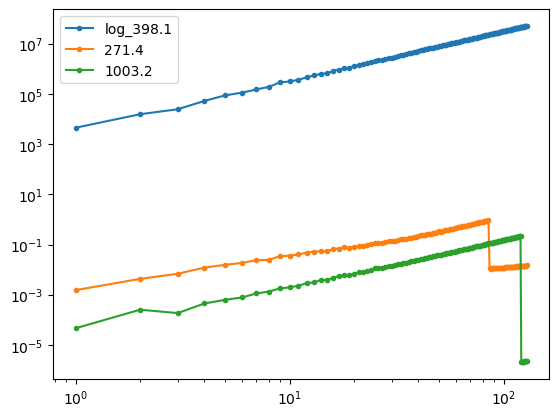
\includegraphics[width=\linewidth]{./figures/polydisperse/log_comp.png}
	\end{center}
\caption[Fluctuations from the logarithmic and the clipped continuity equation]{Comparing fluctuations in of evolution of $g$ in Eq. \eqref{lucky-log-cont} v continuity equation of Eq. \eqref{lucky-3Deqns} and clipping. The fluctuations differ by orders of magnitude and is mostly incorrect. }
\label{lucky-log_comp}
\end{minipage}
\hfill
\begin{minipage}{0.45\textwidth}
    \begin{center}
		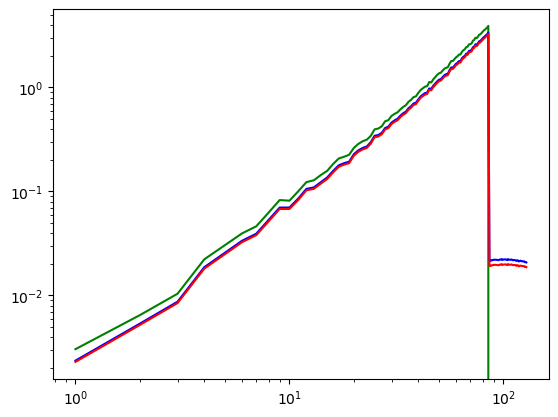
\includegraphics[width=\linewidth]{./figures/polydisperse/comp-cai-v-my-unclipped.png}
	\end{center}
    \caption[Number density spectra for the unclipped field and two clipping schemes]{Comparison of the number density spectra of unclipped (\textcolor{Green}{green}) old clipping mechanism (\textcolor{red}{red}) and that of \cite{cai2024}(\textcolor{blue}{blue}).}
    \label{lucky-comp-cai-v-my-unclipped}
\end{minipage}
\end{figure}

Yet another way, suggested by Rama, is not to clip the number density after it goes to zero, but before that. Once the number-density (which is a continuous variable) dips below the value of $1$ particle in a grid i.e., $n(x) < 1/(\Delta x\Delta y\Delta z)$, impose $n(x)\equiv 0$. This method is rooted in reality, but unfortunately decreases the fluctuations even further, as seen Fig. \ref{lucky-clipping-comp}
\begin{figure}
	\begin{center}
		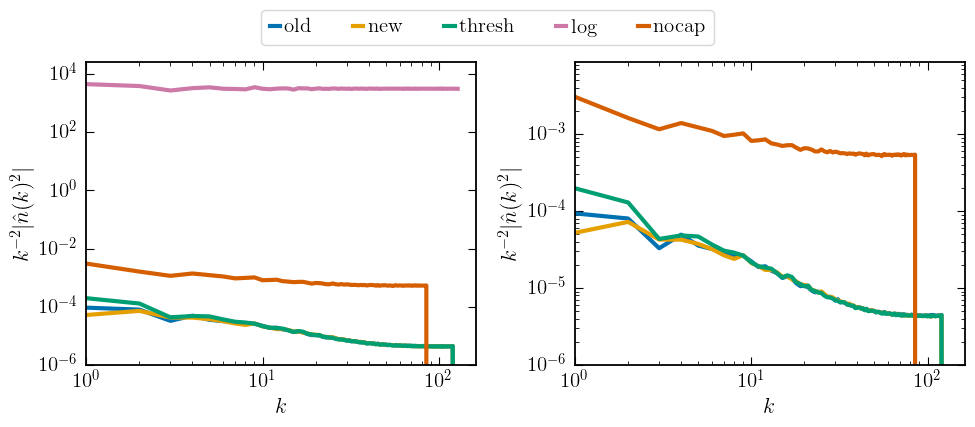
\includegraphics[width=\linewidth]{./figures/polydisperse/clipping-comp.png}
	\end{center}
\caption[Effect of different clipping schemes on number density fluctuations]{Comparing the effects of different clipping on the fluctuations in the number density. New clipping corresponds to the algorithm of \cite{cai2024}. This makes me happy with the old one. In the `nocap' case, 7\% of the number density field is negative. }
\label{lucky-clipping-comp}
\end{figure}

\end{document}
